\documentclass[a4paper, 10pt, ]{article}

\usepackage[slovak]{babel}





\usepackage[utf8]{inputenc}
\usepackage[T1]{fontenc}

\usepackage[left=4cm,
			right=4cm,
            % left=2.5cm,
			% right=5.5cm,
			top=2.1cm,
			bottom=2.6cm,
			footskip=7.5mm,
			% twoside,
			marginparwidth=3.0cm,
			%showframe,
			]{geometry}

\usepackage{graphicx}
\usepackage[dvipsnames]{xcolor}
% https://en.wikibooks.org/wiki/LaTeX/Colors


% ------------------------------

\usepackage{lmodern}

\usepackage[tt={oldstyle=false,proportional=true,monowidth}]{cfr-lm}

% ------------------------------

\usepackage{amsmath}
\usepackage{amssymb}
\usepackage{amsthm}

\usepackage{booktabs}
\usepackage{multirow}
\usepackage{array}
\usepackage{dcolumn}


\usepackage[singlelinecheck=true]{subfig}


% ------------------------------


\def\naT{\mathsf{T}}

\hyphenpenalty=6000
\tolerance=1000




% ------------------------------


\makeatletter

	\def\@seccntformat#1{\protect\makebox[0pt][r]{\csname the#1\endcsname\hspace{4mm}}}

	\def\cleardoublepage{\clearpage\if@twoside \ifodd\c@page\else
	\hbox{}
	\vspace*{\fill}
	\begin{center}
	\phantom{}
	\end{center}
	\vspace{\fill}
	\thispagestyle{empty}
	\newpage
	\if@twocolumn\hbox{}\newpage\fi\fi\fi}

	\newcommand\figcaption{\def\@captype{figure}\caption}
	\newcommand\tabcaption{\def\@captype{table}\caption}

\makeatother


% ------------------------------




\usepackage{fancyhdr}
\fancypagestyle{plain}{%
\fancyhf{} % clear all header and footer fields
\fancyfoot[C]{\sffamily {\bfseries \thepage}\ | {\scriptsize\oznacenieCasti}}
\renewcommand{\headrulewidth}{0pt}
\renewcommand{\footrulewidth}{0pt}}
\pagestyle{plain}


% ------------------------------


\usepackage{titlesec}
\titleformat{\paragraph}[hang]{\sffamily  \bfseries}{}{0pt}{}
\titlespacing*{\paragraph}{0mm}{3mm}{1mm}
\titlespacing*{\subparagraph}{0mm}{3mm}{1mm}

\titleformat*{\section}{\sffamily\Large\bfseries}
\titleformat*{\subsection}{\sffamily\large\bfseries}
\titleformat*{\subsubsection}{\sffamily\normalsize\bfseries}






% ------------------------------

\PassOptionsToPackage{hyphens}{url}
\usepackage[pdfauthor={},
			pdftitle={},
			pdfsubject={},
			pdfkeywords={},
			% hidelinks,
			colorlinks=false,
			breaklinks,
			]{hyperref}


% ------------------------------


\graphicspath{%
{../fig_standalone/}%
{../../PY/fig/}%
{../../PY/jupynotex/fig/}%
{../../ML/fig/}%
{./fig/}%
}



% ------------------------------

\usepackage{enumitem}

\usepackage{lettrine}

% ------------------------------


\usepackage{microtype}


% ------------------------------

\usepackage[titles]{tocloft}

\setlength{\cftsecindent}{-12mm}
\setlength{\cftsecnumwidth}{12mm}
\renewcommand{\cftsecpresnum}{\hfill}
\renewcommand{\cftsecaftersnum}{\hspace{4mm}}

\setlength{\cftsubsecindent}{-12mm}
\setlength{\cftsubsecnumwidth}{16mm} % 12 + 4
\renewcommand{\cftsubsecpresnum}{\hfill}
\renewcommand{\cftsubsecaftersnum}{\hspace{8mm}} % 4 + 4 mm

\setlength{\cftsubsubsecindent}{-12mm}
\setlength{\cftsubsubsecnumwidth}{20mm} % 12 + 4 + 4
\renewcommand{\cftsubsubsecpresnum}{\hfill}
\renewcommand{\cftsubsubsecaftersnum}{\hspace{12mm}} % 4 + 4 + 4 mm

\renewcommand{\cftsecpagefont}{\lstyle \bfseries}
\renewcommand{\cftsubsecpagefont}{\lstyle}
\renewcommand{\cftsubsubsecpagefont}{\lstyle}



\setlength{\cftparaindent}{-16mm}
\setlength{\cftparanumwidth}{28mm} % 16 + 4 + 4 + 4
\renewcommand{\cftparapresnum}{\hfill}
\renewcommand{\cftparaaftersnum}{\hspace{16mm}} % 4 + 4 + 4 + 4 mm








% ------------------------------

\usepackage{listings}



\renewcommand{\lstlistingname}{Výpis kódu}
\renewcommand{\lstlistlistingname}{Výpisy kódu}




%New colors defined below
\definecolor{codegreen}{rgb}{0,0.6,0}
\definecolor{codegray}{rgb}{0.5,0.5,0.5}
\definecolor{codepurple}{rgb}{0.58,0,0.82}
\definecolor{backcolour}{rgb}{0.95,0.95,0.95}

%Code listing style named "mystyle"
\lstdefinestyle{mystyle}{
  backgroundcolor=\color{backcolour},
  commentstyle=\fontfamily{lmtt}\fontsize{8.5pt}{8.75pt}\selectfont\color{codegreen},
  keywordstyle=\fontfamily{lmtt}\fontsize{8.5pt}{8.75pt}\selectfont\bfseries\color{Blue},
  stringstyle=\fontfamily{lmtt}\fontsize{8.5pt}{8.75pt}\selectfont\color{codepurple},
  basicstyle=\fontfamily{lmtt}\fontsize{8.5pt}{8.75pt}\selectfont,
  breakatwhitespace=false,
  breaklines=true,
  captionpos=t,
  keepspaces=true,
  numbers=left,
  numbersep=4mm,
  numberstyle=\fontfamily{lmtt}\fontsize{8.5pt}{8.75pt}\selectfont\color{lightgray},
  showspaces=false,
  showstringspaces=false,
  showtabs=false,
  tabsize=2,
  % xleftmargin=10pt,
  framesep=10pt,
  language=Python,
  escapechar=|,
}


\lstset{
    inputencoding=utf8,
    extendedchars=true,
    literate=%
    {á}{{\'a}}1
    {č}{{\v{c}}}1
    {ď}{{\v{d}}}1
    {é}{{\'e}}1
    {ě}{{\v{e}}}1
    {í}{{\'i}}1
    {ň}{{\v{n}}}1
    {ó}{{\'o}}1
    {ř}{{\v{r}}}1
    {š}{{\v{s}}}1
    {ť}{{\v{t}}}1
    {ú}{{\'u}}1
    {ů}{{\r{u}}}1
    {ý}{{\'y}}1
    {ž}{{\v{z}}}1
    {Á}{{\'A}}1
    {Č}{{\v{C}}}1
    {Ď}{{\v{D}}}1
    {É}{{\'E}}1
    {Ě}{{\v{E}}}1
    {Í}{{\'I}}1
    {Ň}{{\v{N}}}1
    {Ó}{{\'O}}1
    {Ř}{{\v{R}}}1
    {Š}{{\v{S}}}1
    {Ť}{{\v{T}}}1
    {Ú}{{\'U}}1
    {Ů}{{\r{U}}}1
    {Ý}{{\'Y}}1
    {Ž}{{\v{Z}}}1
    {ô}{{\^{o}}}1
}


% ------------------------------


\usepackage{caption}

\DeclareCaptionFormat{odsadene}{\protect\makebox[0pt][r]{#1#2\hspace{4mm}}#3\par}
\DeclareCaptionLabelSeparator{lendvojbodka}{:}
% \DeclareCaptionFont{lightgray}{\color{lightgray}}
\DeclareCaptionFont{lightgray}{\fontfamily{lmtt}\fontsize{8.5pt}{8.75pt}\selectfont\color{lightgray}}

\captionsetup[lstlisting]{format=odsadene, labelsep=lendvojbodka, justification=raggedright, singlelinecheck=false, labelfont={sf, lightgray},}


% ------------------------------





% ------------------------------

\usepackage[backend=biber,
            style=numeric,
            sorting=none,
            ]{biblatex}
\DeclareSourcemap{
    \maps[datatype=bibtex]{
        \map{
        \step[fieldset=note, null]
        }
        \map{
        \step[fieldset=file, null]
        }        
        % \map{
        % \step[fieldset=url, null]        
        % }
        \map{
        \step[fieldset=eprint, null]
        }
    }
}


\addbibresource{E:/_CurrentContent/01_work_repo/bibLaTeXDB/bibLaTeXDB.bib} % nonpublic data





\def\oznacenieCasti{MRS05 - ZS2023}



\usepackage{pdflscape}
\usepackage{longtable}

% \usepackage{afterpage}

\begin{document}


\lstset{%
style=mystyle,
rangebeginprefix=\#\#\#\ cellB\ ,%
rangebeginsuffix=\ \#\#\#,%
rangeendprefix=\#\#\#\ cellE\ ,%
rangeendsuffix=\ \#\#\#,%
includerangemarker=false,
}




\fontsize{12pt}{22pt}\selectfont

\centerline{\textsf{Modelovanie a riadenie systémov} \hfill \textsf{\oznacenieCasti}}

\fontsize{18pt}{22pt}\selectfont






\begin{flushleft}
	\textbf{\textsf{Stabilita,\\prevodová charakteristika\\a~prechodová charakteristika}}
\end{flushleft}





\normalsize

\bigskip

{\hypersetup{hidelinks}

\tableofcontents

}

\bigskip

\vspace{18pt}





\pagebreak

\section{O stabilite dynamického systému}

\lettrine[lines=3, nindent=0pt]{P}{ripomeňme}
% Pripomeňme
matematický model kyvadla, ktorým sme sa zaoberali v predchádzajúcich témach.
Pohybová rovnica opisujúca dynamiku rotačného pohybu kyvadla je v tvare
\begin{align} \label{PohRovKyvadla} %\label{PohRovKyvadlab}
		&ml^2 \ddot{\varphi} = -\beta \dot{\varphi} - mgl\sin{\varphi} + u
\end{align}
pričom ide o kyvadlo, ktorého kmity sú tlmené viskóznym trením s~koeficientom $\beta$ [kg~m$^2$~s$^{-1}$], hmotný bod s~hmotnosťou $m$ [kg] pripevnený na ramene so zanedbateľnou hmotnosťou a~dĺžkou $l$ [m] kmitá okolo osi otáčania a uhol od zvislice je označený $\varphi$ [rad]. $g$~[m~s$^{-2}$] je gravitačné zrýchlenie. Číselné hodnoty parametrov kyvadla sú uvedené v tabuľke~\ref{Parametre kyvadla}.



Ďalej sme uvažovali, že stavom kyvadla sú dve veličiny: uhol natočenia ramena kyvadla $\varphi$ a~uhlová rýchlosť ramena kyvadla $\dot\varphi$. Stavový vektor má preto dva prvky $x^{\mathsf{T}} = \begin{bmatrix} x_1 & x_2	\end{bmatrix}$, kde $x_1 = \varphi$ a~$x_2 = \dot\varphi$. Model kyvadla v stavovom priestore je v tvare
\begin{subequations}
	\begin{align}
		\begin{bmatrix}
			\dot{x}_1 \\ \dot{x}_2
		\end{bmatrix}
		&=
		\begin{bmatrix}
			x_2 \\ - \frac{\beta}{ml^2} x_2 - \frac{g}{l} \sin(x_1)
		\end{bmatrix}
		+
		\begin{bmatrix}
			0 \\ \frac{1}{ml^2}
		\end{bmatrix}
		u \\
		\varphi &= x_1
	\end{align}
\end{subequations}
Toto je nelineárny časovo-invariantný systém druhého rádu.


V tejto časti budeme uvažovať predmetný dynamický systém, avšak bez vstupu, inými slovami externý moment sily je nulový, $u(t) = 0$. Potom
\begin{subequations}
	\begin{align} \label{fajnVektRov}
		\begin{bmatrix}
			\dot{x}_1 \\ \dot{x}_2
		\end{bmatrix}
		&=
		\begin{bmatrix}
			x_2 \\ - \frac{\beta}{ml^2} x_2 - \frac{g}{l} \sin(x_1)
		\end{bmatrix}
 \\
		\varphi &= x_1
	\end{align}
\end{subequations}





\begin{table}[b]
	\centering
	\catcode`\-=12

\caption{Parametre kyvadla}
\label{Parametre kyvadla}
\begin{tabular}{     c    c   c       }
\toprule
Parameter   & Hodnota    & Jednotky              \\
\midrule
$m$       & $1$   & kg             \\
$l$    &  $1$  & m \\
$g$   & $9,81$  & m s$^{-2}$ \\
$\beta$  &  $2 \cdot 0,5 \cdot \sqrt{g/l}$ &  kg~m$^2$~s$^{-1}$ \\
\bottomrule
\end{tabular}
\end{table}


\subsection{Vektorové pole, fázový portrét, ekvilibrium}

Kvalitatívne správanie sa nelineárneho dynamického systému je dôležité pre porozumenie kľúčovým konceptom Lyapunovovej teórie stability systémov. Pre analýzu je dôležitá istá trieda systémov nazývaná planárne dynamické systémy. Tieto systémy majú dve stavové veličiny $x \in \mathbb{R}^2$, čo umožňuje znázorniť stavový priestor v rovine so súradnicovým systémom $(x_1, x_2)$. Navyše výsledky kvalitatívnej analýzy platia vo všeobecnosti a~môžu byť použité aj pri systémoch vyššieho rádu. Preto sú tieto systémy dôležité z hľadiska analýzy. Do tejto triedy systémov patrí aj model kyvadla.

Výhodným spôsobom ako porozumieť správaniu dynamického systému so stavom $x \in \mathbb{R}^2$ je nakresliť \emph{fázový portrét systému}. Začneme zavedením konceptu \emph{vektorového poľa}. Pre systém obyčajných diferenciálnych rovníc zapísaných kompaktne vo vektorovej rovnici (ako rovnica \eqref{fajnVektRov}) v tvare
\begin{align}
	\dot{x} = F(x)
\end{align}
pravá strana rovnice definuje v každom $x \in \mathbb{R}^n$ rýchlosť $F(x) \in \mathbb{R}^n$. Táto rýchlosť hovorí o tom ako sa $x$ mení a~môže byť reprezentovaná vektorom.

Pri planárnom dynamickom systéme, každý stav zodpovedá bodu v rovine a $F(x)$ je vektor rýchlosti reprezentujúci veľkosť a smer zmeny (rýchlosti) daného stavu. Tieto vektory môžme vykresliť na mriežke bodov v rovine a získať tak vizuálny obraz dynamiky systému, tak ako na Obr.~\ref{Vektorové pole znázorňujúce dynamiku kyvadla}. Pre vykreslenie tohto vektorového poľa boli použité parametre kyvadla uvedené v~Tabuľke~\ref{Parametre kyvadla} a tieto parametre budú používané aj v~ďalšom.



\begin{figure}[t]
\centering

	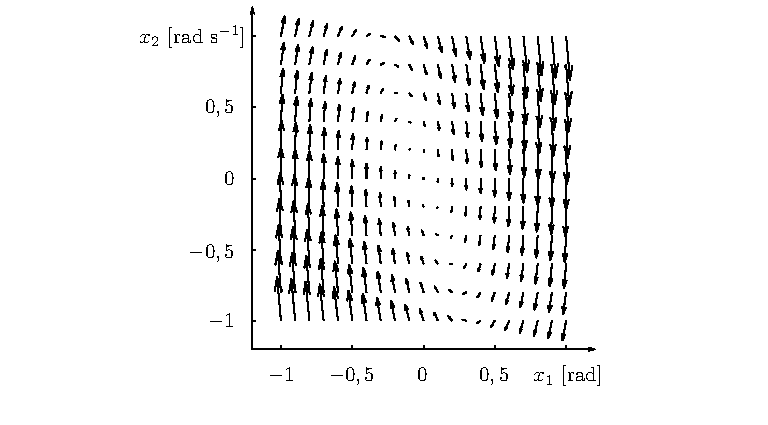
\includegraphics{Obr_KyvydloVektField.pdf}

	\vspace{-7mm}

	\caption{Vektorové pole znázorňujúce dynamiku kyvadla (obrázok vytvorený v~Matlabe, viď text)}

	\label{Vektorové pole znázorňujúce dynamiku kyvadla}
\end{figure}


% \begin{center}
%
%     \makebox[\textwidth][c]{%
% 	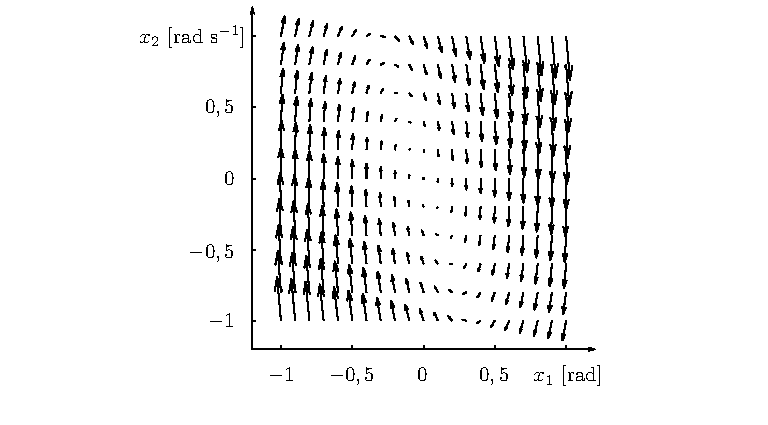
\includegraphics{Obr_KyvydloVektField.pdf}
% 	}
%
% 	\vspace{-7mm}
%
%     \figcaption{Vektorové pole znázorňujúce dynamiku kyvadla (obrázok vytvorený v~Matlabe, viď text)}
% 	\label{Vektorové pole znázorňujúce dynamiku kyvadla}
%
% \end{center}








\paragraph{Vektorové pole}


Vektorové pole na obr.~\ref{Vektorové pole znázorňujúce dynamiku kyvadla} bolo vygenerované v~Matlabe použitím nasledujúceho kódu:
\begin{lstlisting}[language=Matlab, title=Kód pre vygenerovanie obr.~\ref{Vektorové pole znázorňujúce dynamiku kyvadla}]
m = 1; %kg
l = 1; %m
g = 9.81; %m/s^2
beta = 2*0.5*sqrt(g/l); %kgm^2/s
[x1, x2] = meshgrid(-1:.1:1, -1:.2:1);
x1dot = x2;
x2dot = -(beta/m*l^2).*x2 - (g/l).*sin(x1);
quiver(x1,x2,x1dot,x2dot,1.5);
axis([-1.2 1.2 -1.2 1.2])
axis equal
\end{lstlisting}


Body, v ktorých je vektor rýchlosti nulový sú obzvlášť zaujímavé, pretože definujú stacionárne body systému: ak je autonómny systém v~takom stave na začiatku, ostane v tom stave po celý čas.


\paragraph{Fázový portrét}

Fázový portrét (nazývaný aj Fázový diagram) pozostáva z \uv{prúdnic} nakreslených podľa vektorového poľa. Inými slovami, pre istú množinu začiatočných stavov vykreslíme riešenia diferenciálnej rovnice v~rovine a~smer pohybu v stavovom priestore vyznačíme šípkou. To zodpovedá sledovaniu \uv{šípky vektorového poľa} v~každom bode stavového priestoru a nakresleniu výslednej trajektórie. Po vykreslení niekoľkých trajektórii pre rôzne začiatočné stavy získame fázový portrét ako na Obr.~\ref{Fázový portrét kyvadla}.



\begin{figure}[t]
		\centering
        \vspace{-3mm}
		\makebox[\textwidth][c]{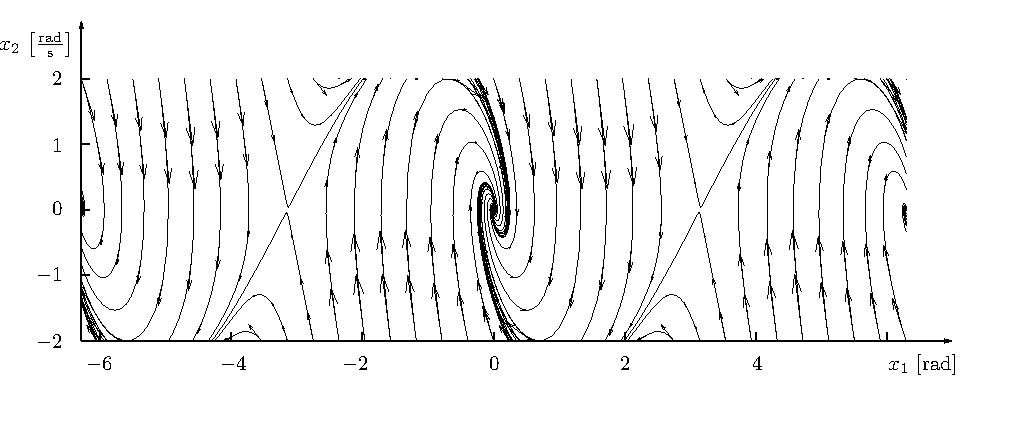
\includegraphics{Obr_KyvadloFazPortret.pdf}}
		\vspace{-10mm}
		\caption{Fázový portrét kyvadla (obrázok vytvorený v Matlabe, viď text pre zdrojový kód)}
		\label{Fázový portrét kyvadla}
		\vspace{-3mm}
\end{figure}




Zdrojový kód pre MATLAB pre získanie tohto obrázku je nasledovný:
\begin{lstlisting}[language=Matlab, title=Kód pre vygenerovanie obr.~\ref{Fázový portrét kyvadla}]
global m l g beta
m = 1; %kg
l = 1; %m
g = 9.81; %m/s^2
beta = 2*0.5*sqrt(g/l); %kgm^2/s

for uhlovarychlost = -2:4:2
  for uhol = -360:22.5:360
    [t,x]=ode45(@PravaStr,[0 5],[uhol*pi/180 uhlovarychlost]);
    hold on
    stav = x;
    x = x(1:5:end-70,:);
    x1dot = x(:,2);
    x2dot=-(beta/m*l^2)*x(:,2)-(g/l)*sin(x(:,1));
    quiver(x(:,1),x(:,2),x1dot,x2dot,0.5,'k')
    plot(stav(:,1),stav(:,2),'k');
    hold off
  end
end

axis equal
axis([-2*pi 2*pi -2 2])
\end{lstlisting}
kde funkcia \verb|PravaStr| je
\begin{lstlisting}[language=Matlab]
function dotx = PravaStr(t,x)
  global m l g beta
  dotx(1)=x(2);
  dotx(2)=-(beta/m*l^2)*x(2)-(g/l)*sin(x(1));
  dotx=dotx';
end
\end{lstlisting}


Fázový portrét je nástroj, ktorý umožňuje posudzovať celkovú dynamiku systému pomocou vykreslenia niekoľkých riešení v stavovom priestore (rovine) systému. Napríklad je možné vidieť, či sa všetky trajektórie s narastajúcim časom približujú k jednému bodu alebo či ide o komplikovanejšie správanie systému. Fázový portrét však nehovorí o veľkosti rýchlosti zmeny stavu (avšak toto môže byť odvodené z dĺžky vektorov vo vektorovom poli systému).


\paragraph{Ekvilibrium}

Ekvilibrium dynamického systému je bod v stavovom priestore, ktorý reprezentuje rovnovážne podmienky pre dynamiku systému. Ide o stacionárny bod, v ktorom je vektor rýchlosti trajektórie systému nulový, ako už bolo uvedené.

Hovoríme, že stav $x_e$ je ekvilibrium dynamického systému
\begin{equation*}
	\dot{x} = F(x)
\end{equation*}
ak $F(x_e) = 0$. Ak má autonómny systém začiatočnú podmienku $x(0) = x_e$, potom ostane v tomto stave a~riešenie má tvar $x(t) = x_e$ po celý čas $t>0$, kde sme uvažovali začiatočný čas $t_0 = 0$.

Stacionárne body (ekvilibriá) patria medzi najdôležitejšiu vlastnosť dynamického systému, pretože definujú stavy s nemennými pracovnými podmienkami systému. Systém môže mať nula, jeden alebo viac stacionárnych bodov.

Stacionárne body uvažovaného kyvadla sú
\begin{equation}
	x_e = \begin{bmatrix} \pm n \pi \\ 0 \end{bmatrix}
\end{equation}
kde $n = 0,1,2,\ldots$. Pre párne $n$ sú to stavy keď kyvadlo visí smerom dole a pre nepárne $n$ je kyvadlo v inverznej polohe. Fázový portrét na Obr.~\ref{Fázový portrét kyvadla} je nakreslený pre $-2\pi \leq x_1 \leq 2\pi$, teda na obrázku je päť stacionárnych bodov.







\subsection{Stabilita dynamického systému vo všeobecnosti}


Pripomeňme, že sa zaoberáme autonómnym systémom (homogénnou diferenciálnou rovnicou) v tvare
\begin{equation} \label{vusetrovanySystem}
	\dot{x} = F(x)
\end{equation}
a tiež pripomeňme, čo rozumieme pod pojmom riešenie systému, alebo skrátene riešenie. Hovoríme, že $x(t)$ je \emph{riešenie} diferenciálnej rovnice \eqref{vusetrovanySystem} na časovom intervale od $t_0 \in \mathbb{R}$ do $t_f \in \mathbb{R}$ ak
\begin{equation}
	\frac{\text{d}x(t)}{\text{d}t} = F \big( x(t)  \big) \qquad \text{pre} \; t_0 < t < t_f
\end{equation}
Daná diferenciálna rovnica môže mať mnoho riešení, najčastejšie nás však zaujíma úloha so zadaným začiatočným stavom, inými slovami so zadanými začiatočnými podmienkami, kedy $x(t)$ je predpísané v začiatočnom čase $t_0$ a úlohou je nájsť riešenie vyhovoujúce pre celý budúci čas $t>t_0$. Vtedy $x(t)$ je riešenie diferenciálnej rovnice \eqref{vusetrovanySystem} so začiatočným stavom $x_0 \in \mathbb{R}^n$ v čase $t_0$ ak
\begin{equation}
	x(t_0) = x_0 \quad \text{a} \quad \frac{\text{d}x(t)}{\text{d}t} = F \big( x(t)  \big) \quad \text{pre} \; t_0 < t < t_f
\end{equation}
Najčastejšie sa stretávame s diferenciálnymi rovnicami, pre ktoré existuje jedinečné riešenie, navyše pre celý čas $t>t_0$ čo znamená že $t_f = \infty$. Častým je tiež, že funkcia $F$ je nezávislá od času, preto môžme uvažovať $t_0 = 0$.



\emph{Stabilita riešenia} určuje či iné riešenia v~blízkosti skúmaného riešenia ostávajú v~jeho blízkosti, približujú sa k~nemu alebo sa od neho vzďaľujú. Uvedieme niekoľko neformálnych a formálnych definícií stability:

\noindent
Nech $x(t;a)$ je riešenie diferenciálnej rovnice so začiatočným stavom $a$. Toto riešenie je stabilné ak iné riešenia, ktoré začínajú v blízkosti $a$ zostávajú v blízkosti $x(t;a)$. Formálne, hovoríme, že riešenie $x(t;a)$ je stabilné ak pre všetky $\epsilon > 0$ existuje $\delta > 0$ taká, že
\begin{equation} \label{stabilDef}
	\left\| b - a \right\| < \delta \; \Rightarrow \; \left\| x(t;b) - x(t;a) \right\| < \epsilon, \; \forall \, t>0
\end{equation}
Všimnime si, že to neznamená, že $x(t;b)$ sa približuje k~$x(t;a)$, len ostáva v jeho blízkom okolí. Navyše hodnota $\delta$ môže závisieť od $\epsilon$, teda napríklad ak chceme ostať blízko nejakého riešenia potom musíme začať veľmi blízko tohto riešenia. Takto definovaná stabilita sa nazýva \emph{stabilita v zmysle Lyapunova}.

Ilustrujeme uvedenú podmienku \eqref{stabilDef} na riešení diferenciálnej rovnice kyvadla \eqref{fajnVektRov}. Začiatočný čas zvoľme $t_0 = 0$ [s], konečný čas zvoľme $t_f = 1,4$ [s], začiatočnú polohu kyvadla zvoľme $\varphi = 45^{\circ}$ a~začiatočná rýchlosť kyvadla nech je nulová. Začiatočný stav v~stavovom priestore je $a = \begin{bmatrix} 0,7854 & 0 \end{bmatrix}^\mathsf{T}$. Týmto začiatočným podmienkam prislúcha riešenie $x(t;a)$, ktoré je znázornené v stavovom priestore na Obr.~\ref{Trajektórie stavu kyvadla v stavovom priestore}, kde je vyznačený aj začiatočný stav $a$. Nebudeme skúmať všetky $\epsilon > 0$, preskúmame len jedno. Napríklad pre $\epsilon = 0,15$ hľadájme $\delta > 0$, ktorá spĺňa podmienku \eqref{stabilDef}. Taká $\delta$ existuje, pretože pre riešenie $x(t;b)$, ktoré začína v stave $b = \begin{bmatrix} 0,8727 & 0 \end{bmatrix}^\mathsf{T}$ platí, že $\left\| x(t;b) - x(t;a) \right\| < \epsilon$, čo je zrejmé z~Obr.~\ref{Trajektórie stavu kyvadla v stavovom priestore} a~aj z~Obr.~\ref{Trajektória rozdielu dvoch riešení daných začiatočnými stavmi }, kde je navyše predĺžený čas riešenia až do nekonečna. Potom sme našli napríklad $\delta = 0,1$ pretože platí
\begin{equation}
	\begin{split}
		\left\| b - a \right\| &= \sqrt{(0,8721 - 0,7854)^2 + (0 - 0)^2} = \\
		&= 0,0873 < 0,1
	\end{split}
\end{equation}
čo je tiež zrejmé najmä z~Obr.~\ref{Trajektória rozdielu dvoch riešení daných začiatočnými stavmi }. Týmto sme nezistili nič o~stabilite riešenia $x(t;a)$, pretože sme neoverili, či je podmienka \eqref{stabilDef} splnená pre všetky $\epsilon > 0$.




\begin{figure}[t]
	\centering
	\makebox[\textwidth][c]{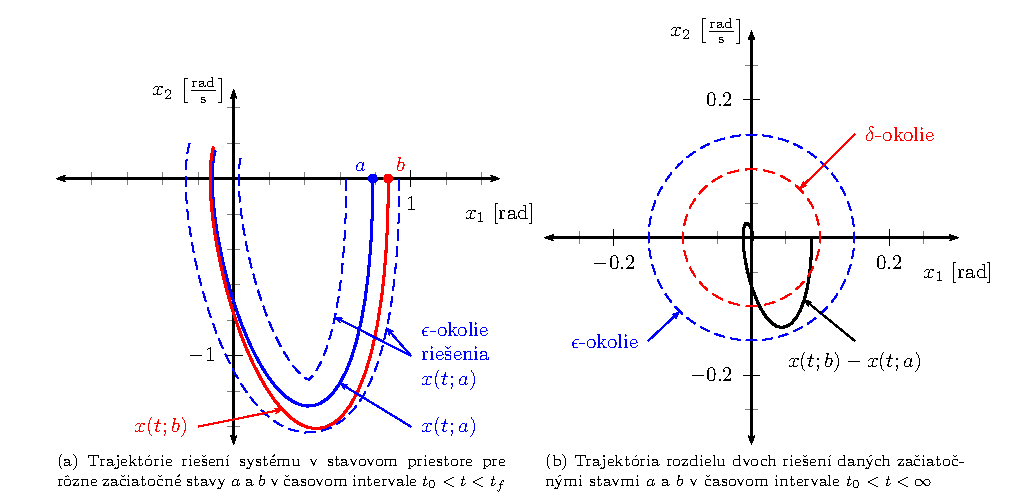
\includegraphics{Obr_LyapTraj.pdf}}

	\subfloat[]{\label{Trajektórie stavu kyvadla v stavovom priestore}}%
	\subfloat[]{\label{Trajektória rozdielu dvoch riešení daných začiatočnými stavmi }}%

		\vspace{-10mm}
	\caption{Ilustračný príklad k definícii stability riešenia systému}
	\label{Ilustračný príklad k definícii stability riešenia systému}
	%\vspace{-5mm}
\end{figure}








Ak je riešenie stabilné v zmysle Lyapunova, ale trajektórie okolitých riešení k nemu nekonvergujú, hovoríme, že riešenie je \emph{neutrálne stabilné}.

Riešenie $x(t;a)$ je \emph{asymptoticky stabilné} ak je stabilné v~zmysle Lyapunova a~zároveň $x(t;b) \to x(t;a)$ s~rastúcim časom $t \to \infty$ pri začiatočnom stave $b$, ktorý je dostatočne blízko stavu~$a$.

Veľmi dôležitým špeciálnym prípadom je ak pre skúmané riešenie platí $x(t;a) = x_e$. Potom nehovoríme o stabilite riešenia ale o~\emph{stabilite stacionárneho bodu}. Príkladom asymptoticky stabilného stacionárneho bodu sú body
\begin{align*}
	x_{e_{-2}} =
	\begin{bmatrix}
		-2\pi \\ 0
	\end{bmatrix},
	\quad
	x_{e_{0}} =
	\begin{bmatrix}
		0 \\ 0
	\end{bmatrix},
	\quad
	\text{a}
	\quad
	x_{e_{2}} =
	\begin{bmatrix}
		2 \pi \\ 0
	\end{bmatrix}
\end{align*}
na Obr.~\ref{Fázový portrét kyvadla}, vidíme, že ak začíname blízko asymptoticky stabilného stacionárneho bodu, s narastajúcim časom sa k nemu približujeme.

Riešenie $x(t;a)$ je \emph{nestabilné} ak nie je stabilné. Konkrétnejšie, hovoríme, že riešenie $x(t;a)$ je nestabilné ak pre akékoľvek dané $\epsilon > 0$ neexistuje $\delta > 0$ taká, že ak $\left\| b - a \right\| < \delta \; \text{potom} \; \left\| x(t;b) - x(t;a) \right\| < \epsilon, \; \forall \, t>0$. Príkladom nestabilného stacionárneho bodu sú body
\begin{align*}
	x_{e_{-1}} =
	\begin{bmatrix}
		-\pi \\ 0
	\end{bmatrix},
	\quad
	\text{a}
	\quad
	x_{e_{1}} =
	\begin{bmatrix}
		\pi \\ 0
	\end{bmatrix}
\end{align*}
na Obr.~\ref{Fázový portrét kyvadla}.

Predchádzajúce definície nezohľadňujú oblasť, na ktorej môžu byť použité. Presnejšie je definovať riešenie ako \emph{lokálne stabilné} (alebo \emph{lokálne asymptoticky stabilné}) ak je stabilné pre všetky začiatočné stavy $x \in B_r(a)$, kde $B_r(a) = \left\{ x \, : \, \| x - a \| < r \right\}$ je oblasť s polomerom $r > 0$ okolo bodu $a$. Riešenie je \emph{globálne stabilné} ak je stabilné pre všetky $r > 0$.












\begin{figure}[!ht]
	\centering

	\subfloat[Fázový portrét nelineárneho modelu kyvadla]{%\label{Trajektórie stavu kyvadla v stavovom priestore}%
		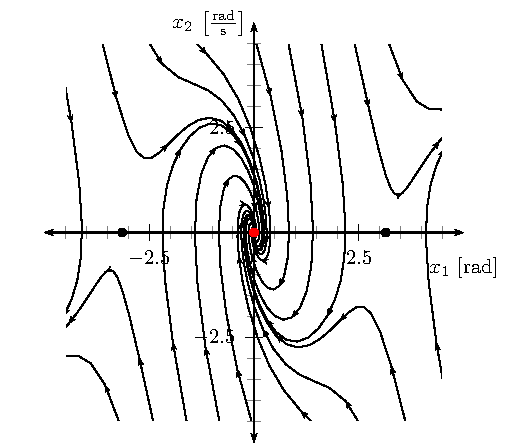
\includegraphics{Obr_FazPorNelin.pdf}
	}
	\hspace{1cm}
	\subfloat[Fázový portrét lineárneho modelu kyvadla]{%\label{Trajektórie stavu kyvadla v stavovom priestore}%
		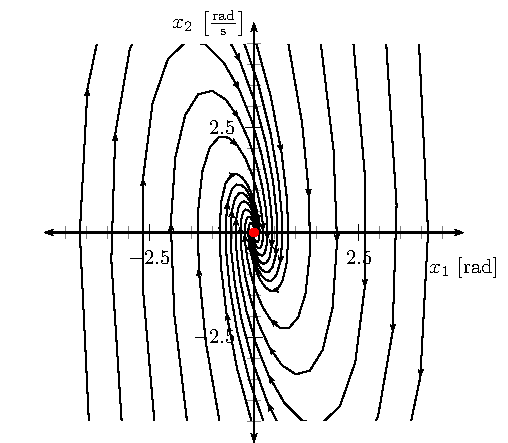
\includegraphics{Obr_FazPorLin.pdf}
	}

	\caption{Porovnanie fázových portrétov nelineárneho systému a jeho linearizovanej aproximácie}
	\label{Porovnanie fázových portrétov nelineárneho systému a jeho linearizovanej aproximácie}
\end{figure}













\subsection{Stabilita lineárnych dynamických systémov}


Lineárny dynamický systém má tvar
\begin{equation}
	\dot{x} = A x, \quad x(0) = x_0
\end{equation}
kde $A \in \mathbb{R}^{n\times n}$ je štvorcová matica. Začiatok stavového priestoru je vždy stacionárnym bodom lineárneho systému a stabilita tohto stacionárneho bodu môže byť určená pomocou vlastných čísel matice $A$.

Vlastné čísla $\lambda(A)$ sú korene \emph{charakteristického polynómu} systému $\det(sI - A)$, kde $s \in \mathbb{C}$ je komplexná premenná a $I$ je jednotková matica. Konkrétne vlastné číslo ($i$-te vlastné číslo) označujeme $\lambda_i$, pričom $\lambda_i \in \lambda(A)$.
%Vo všeobecnosti je vlastné číslo matice $A$ $\lambda_i$ komplexné číslo a keď $A$ obsahuje len reálne čísla potom aj komlexne združené $\lambda_i^*$ je tiež vlastným číslom matice~$A$.

Pre lineárny systém stabilita stacionárneho bodu (ako veľmi dôležitého špeciálneho prípadu spomedzi všetkých riešení) závisí len od matice $A$, čo znamená, že stabilita je vlastnosť systému. Pre lineárny systém preto hovoríme o stabilite systému namiesto o~stabilite konkrétneho riešenia alebo ekvilibria.

Stabilitu lineárneho systému možno zhrnúť do jednej vety:

{ \it
\noindent
Systém
\begin{equation*}
	\dot{x} = A x
\end{equation*}
je asymptoticky stabilný vtedy a len vtedy keď reálne časti všetkých vlastných čísel matice $A$ sú záporné a systém je nestabilný keď aspoň jedno vlastné číslo matice $A$ má kladnú reálnu časť.
}





















\subsubsection{Linearizácia a jej použitie pri analýze stability}
\label{Linajejpouz}


Výhodnou vlastnosťou diferenciálnych rovníc je, že je často možné určiť lokálnu stabilitu stacionárneho bodu pomocou aproximácie nelineárneho systému lineárnym systémom.

Uvažujme nelineárny systém
\begin{align}
	\dot{x} = F(x)
\end{align}
ktorý má ekvilibrium v bode $x_e$. Zaujíma nás stabilita tohto stacionárneho bodu. Aproximujme (linearzujme) nelineárnu funkciu $F(x)$ v okolí bodu $x_e$ pomocou prvých dvoch členov Taylorvho radu
\begin{align}
	F(x) \approx F(x_e) + \left. \frac{\partial F}{\partial x} \right|_{x_e} (x - x_e)
\end{align}
Platí $F(x_e) = 0$, a zavedieme nový stavový vektor $z = x - x_e$. To znamená, že $x = z + x_e$, potom $\dot{x} = \dot{z} + \dot{x}_e$, avšak $x_e$ sa s časom nemení a preto platí  $\dot{x} = \dot{z}$. Lineárna aproximácia pôvodného nelineárneho systému v~okolí bodu $x_e$ má potom tvar
\begin{align}
	\dot{z} = Az
\end{align}
kde
\begin{align} \label{matApoLinearizacii}
	A = \left. \frac{\partial F}{\partial x} \right|_{x_e}
\end{align}

V prípade kyvadla je nelineárny model systému v~tvare \eqref{fajnVektRov} a teda
\begin{align}
	x=
	\begin{bmatrix}
		{x}_1 \\ {x}_2
	\end{bmatrix}
	;
	\;
	F=
	\begin{bmatrix}
		F_1 \\ F_2
	\end{bmatrix}
	=
	\begin{bmatrix}
		x_2 \\ - \frac{g}{l} \sin(x_1) - \frac{\beta}{ml^2} x_2
	\end{bmatrix}
\end{align}
Linearizujme nelineárny model systému \eqref{fajnVektRov} v okolí rovnovážneho stavu $x_e = \begin{bmatrix} 0 & 0 \end{bmatrix}^\mathsf{T}$. Kľúčovým je výpočet matice $A$ podľa \eqref{matApoLinearizacii}. V tomto prípade máme
\begin{align} \label{lineF}
	%\begin{split}
	\frac{\partial F}{\partial x}
	=
	\begin{bmatrix}
		\displaystyle\frac{\partial}{\partial x_1} \left( F_1 \right) & \displaystyle\frac{\partial}{\partial x_2} \left( F_1 \right) \\
		\displaystyle\frac{\partial}{\partial x_1} \left( F_2 \right) & \displaystyle\frac{\partial}{\partial x_2} \left( F_2 \right)
	\end{bmatrix}
	=
	\begin{bmatrix}
		0 & 1 \\
		- \displaystyle\frac{g}{l} \cos(x_1) & - \displaystyle\frac{\beta}{ml^2}
	\end{bmatrix}
%\end{split}
\end{align}
Po dosadení hodnôt stacionárneho bodu za $x_1 = 0$ (a~$x_2 = 0$) do \eqref{lineF} máme
\begin{align}
	A = \left. \frac{\partial F}{\partial x} \right|_{x_e}
	=
	\begin{bmatrix}
		0 & 1 \\
		- \displaystyle\frac{g}{l}  & - \displaystyle\frac{\beta}{ml^2}
	\end{bmatrix}
\end{align}
a vzľadom na fakt, že v tomto prípade $x_e = 0$ je linearizovaný model systému v tvare
\begin{align} \label{vyslednyLinearnyModel}
	\begin{bmatrix}
		\dot{x}_1 \\ \dot{x}_2
	\end{bmatrix}
	=
	\begin{bmatrix}
		0 & 1 \\
		- \displaystyle\frac{g}{l}  & - \displaystyle\frac{\beta}{ml^2}
	\end{bmatrix}
	\begin{bmatrix}
		{x}_1 \\ {x}_2
	\end{bmatrix}
\end{align}

Lokálna stabilita stacionárneho bodu nelineárneho systému teraz môže byť určená pomocou vlastných čísel matice $A$.





Mimochodom výsledný lineárny model \eqref{vyslednyLinearnyModel} je rovnaký, ako keby sme uvažovali, len malé výchylky kyvadla (malé hodnoty uhla $\varphi$), pri ktorý dostatočne presne platí, že $\sin(\varphi) = \varphi$ (angl. Small-angle approximation).

Skutočnosť, že lineárny model môže byť použitý pre opis správania nelineárneho systému v~okolí rovnovážneho stavu je veľmi výhodná. Je to možné využiť aj pre návrh spätnoväzbového regulátora, ktorý udržiava stav nelineárneho systému v okolí rovnovážneho stavu. Pritom samotný regulátor je navrhnutý pre lineárnu aproximáciu systému. Keďže stav systému je regulátorom udržiavaný blízko stacionárneho bodu, tak aj lineárna aproximácia použitá pri stabilizácii je dostatočne presná.

Na Obr.~\ref{Porovnanie fázových portrétov nelineárneho systému a jeho linearizovanej aproximácie} je porovnanie fázových portrétov nelineárneho modelu kyvadla a~linearizovaného modelu kyvadla v okolí začiatku stavového priestoru. Všimnime si, že v~okolí stacionárneho bodu (začiatku súradnicového systému) sú tieto fázové portréty takmer identické.







% \subsection{Späť k nehomogénnemu dynamickému systému\protect\footnote{Taký, čo má vstupný signál.}}
\subsection{Späť k nehomogénnemu dynamickému systému}




Cieľom v tejto časti je prepojiť dosiaľ uvedené s pojmami vstupný signál dynamického systému, stavové veličiny (stav) a stavový priestor, a v neposlednom rade, prenosová funkcia.

Prenosová funkcia opisuje lineárny dynamický systém. Ak je dynamický systém nelineárny, pri istých podmienkach je ho možné linearizovať. Výsledok linearizácie, avšak, len aproximuje vlastnosti pôvodného systému, a čo je najdôležitejšie, iba v~istom (malom) okolí zvoleného bodu v~stavovom priestore.

Dôvodom pre linearizáciu a následnú možnosť mať k dispozícii prenosovú funkciu je zjednodušenie ďalšej práce a využitia samotného modelu systému. Ak je model nelineárny, väčšinou je značne náročné ďalej s ním pracovať -- napríklad teoreticky ho využívať pri návrhu riadiaceho systému. Lineárny model je značne jednoduchšie využívať vo všeobecnosti a napríklad klasická teória automatického riadenia je prirodzene založená na lineárnych dynamických systémoch.

Prenosová funkcia tiež súvisí s Laplaceovou transformáciou, ktorá vo všeobecnosti uľahčuje hľadanie analytického riešenia lineárnej diferenciálnej rovnice opisujúcej spravanie dynamického systému.


\subsubsection{Nelinearita a linearizácia}

Kyvadlo, ktoré sa tu uvádza, možno označiť ako nelineárny dynamický systém. Dôvodom je, že nie je možné nájsť lineárnu funkciu, ktorá by dávala do vzájomného vzťahu časovú deriváciu stavu kyvadla a samotný stav kyvadla.

V prípade kyvadla je celkom prirodzené, že stavovými veličinami sú uhol natočenia ramena kyvadla $\varphi(t)$ a~uhlová rýchlosť ramena kyvadla $\dot\varphi(t)$. Ako už bolo uvedené, vedie to na sústavu diferenciálnych rovníc v tvare
% \begin{subequations}
	\begin{align} \label{nelinSustavaKyvadla}
		\begin{bmatrix}
			\dot{x}_1(t) \\ \dot{x}_2(t)
		\end{bmatrix}
		&=
		\begin{bmatrix}
			x_2(t) \\ - \frac{\beta}{ml^2} x_2(t) - \frac{g}{l} \sin(x_1(t))
		\end{bmatrix}
		+
		\begin{bmatrix}
			0 \\ \frac{1}{ml^2}
		\end{bmatrix}
		u(t)
	\end{align}
% \end{subequations}
kde je zavedené označenie $x_1(t) = \varphi(t)$ a $x_2(t) = \dot\varphi(t)$. Rovnica \eqref{nelinSustavaKyvadla} by sa dala zovšeobecnene vyjadriť v tvare
\begin{equation}
    \dot x(t) = F\left(x(t)\right) + b\,u(t)
\end{equation}
kde $x(t)$ je stavový vektor $x(t) = \begin{bmatrix} x_1(t) & x_2(t) \end{bmatrix}^\mathsf{T}$, ďalej $b$ je jednoducho vektor čísiel, konkrétne $b = \begin{bmatrix} 0 & \frac{1}{ml^2} \end{bmatrix}^\mathsf{T}$ a $F\left(x(t)\right)$ je všeobecná funkcia, ktorej argumentom je predovšetkým stav systému. Výraz $b\,u(t)$ je, samozrejme, lineárny. Všeobecná funkcia $F\left(x(t)\right)$ v tomto prípade nie je lineárna. Ak by bola lineárna bolo by ju možné zapísať v tvare $A\,x(t)$, kde $A$ je matica čísiel. Výraz $\sin(x_1(t))$ však neumožňuje takýto lineárny zápis (vzťah).




\paragraph{Linearizácia}

Ak chceme linearizovať systém, vždy je potrebné uviesť pri akých podmienkach bude táto linearizácia dobrou aproximáciou pôvodného nelieárneho systému. Tu sa na špecifikáciu takýchto podmienok pozerajme z hľadiska bodu v stavovom priestore. Nech je cieľom linearizovať systém v okolí stavu $x(t) = \begin{bmatrix} 0 & 0 \end{bmatrix}^\mathsf{T}$, teda aj poloha aj uhlová rýchlosť kyvadla sú nulové (blízke nule). Nepriamo to udáva, že aj vstup (vstupný moment sily) $u(t) = 0$.

Týmto sú jasne stanovené podmienky, pri ktorých bude linearizácia dobrou náhradou za pôvodný systém -- teda v okolí akého bodu v stavovom priestore, alebo aj v akej, takpovediac, pracovnej oblasti, pričom sa má na mysli hodnota výstupnej veličiny a vstupnej veličiny (tieto hodnoty udávajú tzv. pracovný bod).

Mimochodom, uvedené je z hľadiska výsledku taká istá myšlienka, ako keď sa uvažuje o~aproximácii rovnice kyvadla pre tzv. malé uhly -- vtedy sa jednoducho píše $\sin(x_1(t)) \approx x_1(t)$




Keďže sme sa rozhodli linearizovať pri podmienkach $x(t) = \begin{bmatrix} 0 & 0 \end{bmatrix}^\mathsf{T}$ a $u(t) = 0$, tak výsledok je samozrejme to isté ako je uvedené v časti~\ref{Linajejpouz}.

Tu je totiž cieľom dať do súvisu opis v stavovom priestore a prenosovú funkciu, nie uviesť celý zovšeobecný postup linearizácie.

Lineárne diferenciálne rovnice opisujúce predmetný systém teda v tomto prípade sú rovnaké ako uvádza \eqref{vyslednyLinearnyModel}. Tu však pridajme aj člen so vstupným signálom, aby bolo možné mať aj nenulový vstup -- avšak jeho hodnoty by mali ostať v okolí nuly. Lineárny dynamický systém potom je v tvare
\begin{subequations} \label{vyslednyLinearnyModelajU}
    \begin{align}
    	\begin{bmatrix}
    		\dot x_1(t) \\ \dot x_2(t)
    	\end{bmatrix}
    	&=
    	\begin{bmatrix}
    		0 & 1 \\
    		- \displaystyle\frac{g}{l}  & - \displaystyle\frac{\beta}{ml^2}
    	\end{bmatrix}
    	\begin{bmatrix}
    		x_1(t)\\ x_2(t)
    	\end{bmatrix}
        +
        \begin{bmatrix}
    		0\\ \frac{1}{ml^2}
    	\end{bmatrix}
        u(t)
        \\
        y(t) &= x_1(t)
    \end{align}
\end{subequations}
kde $y(t)$ predstavuje zavedenie výstupnej veličiny systému -- poloha kyvadla je výstupnou veličinou.

Sústavu diferenciálnych rovníc možno všeobecnejšie zapísať ak nepoužijeme konkrétne parametre $m$, $l$, $\beta$ a $g$, ale všeobecné koeficienty:
\begin{subequations}
    \begin{align}
    	\dot x(t)
    	&=
    	\begin{bmatrix}
    		0 & 1 \\
    		- a_0  & - a_1
    	\end{bmatrix}
    	x(t)
        +
        \begin{bmatrix}
    		0\\ b_0
    	\end{bmatrix}
        u(t)
        \\
        y(t) &= \begin{bmatrix} 1 & 0 \end{bmatrix} x(t)
    \end{align}
\end{subequations}
kde sme rovno písali stavový vektor $x(t)$. Toto je zjavne lineárna rovnica, presnejšie, sústava lineárnych dynamických rovníc. Týmto samozrejme smerujeme k zápisu v~tvare
\begin{subequations} \label{ldsvovsp}
    \begin{align}
    	\dot x(t) &= A x(t) + b u(t) \label{srvovsp} \\
        y(t) &= c^\mathsf T x(t)
    \end{align}
\end{subequations}





\subsubsection{Prenosová funkcia (pre úplnosť)}
\label{tdopiscast}

Cieľom je tu prezentovať intuitívny pohľad na prevod lineárneho dynamického systému s opisu v stavovom priestore, ako je~\eqref{ldsvovsp}, na prenosovú funkciu.

Laplaceov operátor $s$ aplikovaný na signál má rovnaký význam ako časová derivácia aplikovaná na signál. Formálnejšie: majme signál $z(t)$ a keď napíšeme $s\, z(t)$ myslí sa tým to isté ako by sme napísali $\dot z(t)$ alebo teda $\frac{\text{d}}{\text{d}t} z(t)$.

Píšme rovnicu \eqref{srvovsp} tak, že deriváciu nahradíme operátorom $s$.
\begin{align}
    s x &= A x + b u
\end{align}
Použitie operátora $s$ má istý vplyv na samotné signály, tu to však nie je podstatné, len to zohľadňujeme tým, že signály tu neznačíme ako funkciu času (píšeme len $x$, nie $x(t)$).

Prenosová funkcia je (z definície) pomer výstupného ku vstupnému signálu. Vstupom tu je jednoznačne $u$, preto by bolo výhodné dostať všetky $x$ na ľavú stranu a osamostatniť tento signál (stavový vektor). Môžme písať
\begin{align}
    s x - A x  &=  b u
\end{align}
Avšak, ak teraz chceme osamostatniť $x$, je potrebné dávať pozor na rozmery členov rovnice. Matica $A$ ma rozmer $2\times2$. Preto zaveďme výraz $sI$, kde $I$ je jednotková matica s~práve takým rozmerom a teda $sI$ je matica, ktorá má na diagonále operátori~$s$. Potom môžeme písať
\begin{align}
    \left(sI - A\right) x  &=  b u
\end{align}
Výraz $\left(sI - A\right)$ je štvorcová matica. Pre osamostatnenie $x$ na ľavej strane rovnice je potrebné z ľava prenásobiť rovnicu inverziou tejto matice. Teda
\begin{align}
     x  &=  \left(sI - A\right)^{-1} b u
\end{align}
Všimnime si, že stále platí, že na ľavej aj pravej strane je výraz, ktorý má rozmer $2\times1$ (vektor $x$ má takýto rozmer).

Cieľom je však získať pomer výstupného ku vstupnému signálu. Výstupným signálom je $y$, pre ktorý platí $y = c^\mathsf T x$. Preto potom
\begin{align}
     y  &=  c^\mathsf T\left(sI - A\right)^{-1} b u
\end{align}
a teda
\begin{align} \label{tfifoss}
     \frac{y}{u} &=  c^\mathsf T\left(sI - A\right)^{-1} b
\end{align}

Výraz na pravej strane rovnice \eqref{tfifoss} je prenosová funkcia -- stačí dosadiť konkrétne matice, v tomto prípade to v podstate znamená:
\begin{subequations}
    \begin{align}
        \frac{y}{u} &=
        \begin{bmatrix} 1 & 0 \end{bmatrix}
        \left(
            \begin{bmatrix} s & 0 \\ 0 & s \end{bmatrix} - \begin{bmatrix} 0 & 1 \\ -a_0 & -a_1 \end{bmatrix}
        \right)^{-1}
        \begin{bmatrix} 0 \\ b_0 \end{bmatrix}
        \\
        \frac{y}{u} &=
        \begin{bmatrix} 1 & 0 \end{bmatrix}
        % \left(
            \begin{bmatrix} s & -1 \\ a_0 & (s+a_1) \end{bmatrix} ^{-1}
        % \right)^{-1}
        \begin{bmatrix} 0 \\ b_0 \end{bmatrix}
    \end{align}
\end{subequations}
Je potrebné urobiť inverziu matice:
\begin{subequations}
    \begin{align}
            \begin{bmatrix} s & -1 \\ a_0 & (s+a_1) \end{bmatrix} ^{-1}
            &=
            \frac{1}{s \left(s + a_1\right) + a_0}
            \begin{bmatrix} (s+a_1) & 1 \\ -a_0 & s \end{bmatrix} \\
            &=
            \frac{1}{s^2 + a_1 s + a_0}
            \begin{bmatrix} (s+a_1) & 1 \\ -a_0 & s \end{bmatrix} \\
            &=
            \begin{bmatrix} \displaystyle \frac{(s+a_1)}{s^2 + a_1 s + a_0} & \displaystyle \frac{1}{s^2 + a_1 s + a_0} \\ \displaystyle \frac{-a_0}{s^2 + a_1 s + a_0} & \displaystyle \frac{s}{s^2 + a_1 s + a_0} \end{bmatrix}
    \end{align}
\end{subequations}
Potom je možné pokračovať v úprave prenosovej funkcie:
\begin{subequations}
    \begin{align}
        \frac{y}{u} &=
        \begin{bmatrix} 1 & 0 \end{bmatrix}
        \begin{bmatrix} \displaystyle \frac{(s+a_1)}{s^2 + a_1 s + a_0} & \displaystyle \frac{1}{s^2 + a_1 s + a_0} \\ \displaystyle \frac{-a_0}{s^2 + a_1 s + a_0} & \displaystyle \frac{s}{s^2 + a_1 s + a_0} \end{bmatrix}
        \begin{bmatrix} 0 \\ b_0 \end{bmatrix} \\
        \frac{y}{u} &=
        \begin{bmatrix} 1 & 0 \end{bmatrix}
        \begin{bmatrix} \displaystyle \frac{b_0}{s^2 + a_1 s + a_0} \\ \displaystyle \frac{b_0 s}{s^2 + a_1 s + a_0} \end{bmatrix} \\
        \frac{y}{u} &=
        \frac{b_0}{s^2 + a_1 s + a_0}
    \end{align}
\end{subequations}
To je, ako sme uviedli, prenosová funkcia. Teraz je zrejmé, že signály na ľavej strane rovnice ($y$ a $u$) sú z formálneho hľadiska tzv. Laplaceove obrazy pôvodných časových signálov -- to ale nebolo pri uvedenej prezentácii podstatné hneď od začiatku.




























\section{O meraní prevodovej charakteristiky}

% \begin{itemize}[leftmargin=0pt, labelsep=4mm, itemsep=0pt]
%     \color{Gray}

%     \item Ponechajme si tu názov časti, že „O meraní\ldots“ aj keď v dobe rúškovej sa nerealizuje meranie, len simulácia\ldots

% \end{itemize}

\noindent
Prevodová charakteristika je závislosť ustálených hodnôt výstupnej veličiny od ustálených hodnôt vstupnej veličiny. Zhruba povedané. Prevodová charakteristika, niekde sa nazýva aj statická charakteristika, teda charakterizuje systém len v~ustálených stavoch. Neobsahuje informáciu o dynamike systému.

V nasledujúcom sa pokúsime načrtnúť meranie prevodovej charakteristiky - tu sa však nebude naozaj niečo merať, ale reálny systém bude nahradený simulovaným. Proces získavania „surových“ dát, ktoré sú potrebné pre určenie prevodovej charakteristiky a proces spracovania týchto dát bude však rovnaký akoby išlo o reálny systém.

Systém, ktorý bude predmetom skúmania, ktorého prevodovú charakteristiku budeme merať, je kyvadlo, tak ako bolo už skôr opísané. Navyše však bude k výstupnej veličine simulováného systému pridaný čitateľovi neznámy šum. Dôvodom je lepšie napodobenie situácie v akej by bol čitateľ ak by sa zaoberal výstupnou veličinou reálneho systému.

















\subsection{Surové dáta \ldots}

Ako už bolo uvedené, predmetom záujmu sú ustálené hodnoty výstupného signálu. Ak na vstup privedieme vstupný signál s nejakou konštantnou vstupnou hodnotou, následne počkáme istý čas nech sa výstupný signál ustáli, tak potom môžeme odčítať (odmerať) ustálenú hodnotu výstupného signálu. Takto sa získa jeden bod z prevodovej charakteristiky.

Hneď potom je však možné zmeniť hodnotu vstupného signálu a opäť čakať, kým sa výstup ustáli.








% \begin{center}

	\begin{figure}[t]
	\centering

    \makebox[\textwidth][c]{%
	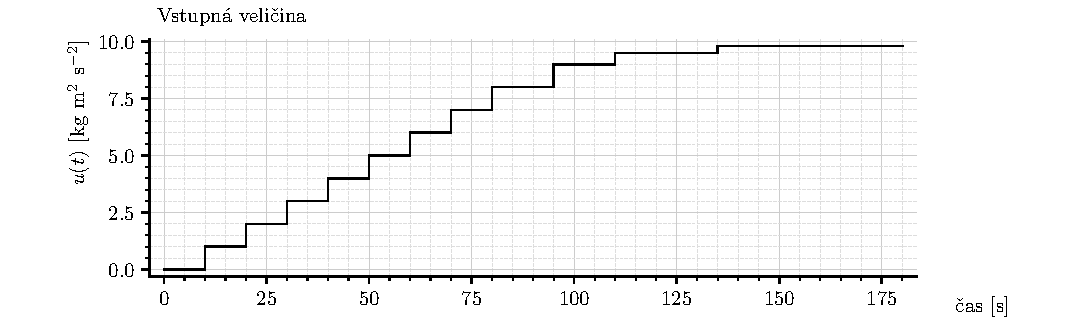
\includegraphics{MRS04_figsc_01_1.pdf}
	}

	\vspace{-6pt}

	\figcaption{Priebeh vstupného signálu}
	\label{Priebeh vstupného signálu}

	\vspace{-6pt}

	\end{figure}

% \end{center}








\begin{table}[b]
	\centering
	\catcode`\-=12

\caption{Hodnoty vstupného signálu}
\label{Hodnoty vstupného signálu}
\begin{tabular}{     c      c       }

\toprule
čas [s] & hodnota [kg m$^2$ s$^{-2}$] \\
\midrule
$0$ & $0,0$ \\
$10$ & $1,0$ \\
$30$ & $2,0$ \\
$20$ & $3,0$ \\
$40$ & $4,0$ \\
$50$ & $5,0$ \\
$60$ & $6,0$ \\
$70$ & $7,0$ \\
$80$ & $8,0$ \\
$95$ & $9,0$ \\
$110$ & $9,5$ \\
$135$ & $9,81$ \\
\bottomrule
\end{tabular}
\end{table}







% \begin{center}

	\begin{figure}[t]
	\centering


    \makebox[\textwidth][c]{%
	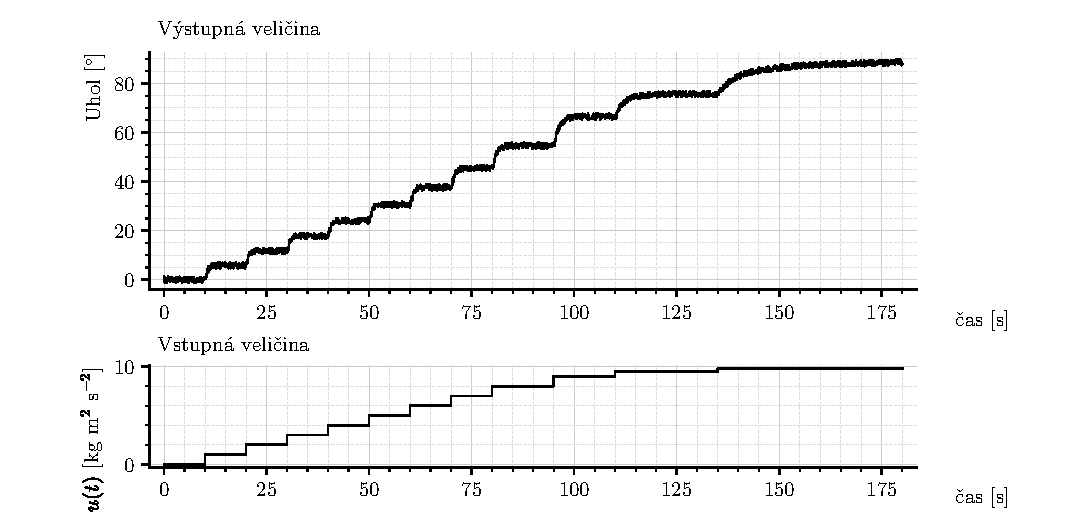
\includegraphics{MRS04_figsc_02_2.pdf}
	}

	\figcaption{Surové dáta. Poznámka: výstupná veličina na obr.~\ref{Surové dáta} je schválne „zašumená“. Napodobňujeme tu tým potenciálny šum snímača, ktorý meria danú veličinu. Dôvodom je najmä skutičnosť, že sa tak lepšie ilustrujú jednotlivé kroky potrebné pre všeobecné spracovanie nameraného signálu, ktoré sú uvedené v ďalších častiach.}
	\label{Surové dáta}

	\end{figure}

% \end{center}






% \afterpage{\clearpage}




Tento postup, hodnoty vstupného signálu a doby, počas ktorých sa „čaká“ na ustálenie výstupu, možno vyjadriť tabuľkou nasledovne. Prvý stĺpec je čas, v ktorom sa zmení (prepne) vstup a druhý stĺpec je hodnota (konštanta), na ktorú sa zmení (prepne).




Z uvedeného je zároveň jasné, že interval vstupných hodnôt, pre ktorý zisťujeme ustálené hodnoty výstupu je $0$ až $9,81$ [kg m$^2$ s$^{-2}$]. Iné by vzhľadom na konkrétne kyvadlo, ktoré sa tu uvažuje, malo pramalý význam.

Vstupný signál tak ako je definovaný tabuľkou~\ref{Hodnoty vstupného signálu} možno znázorniť ako na obr.~\ref{Priebeh vstupného signálu}.


Simulujme teraz priebeh výstupnej veličiny kyvadla (výchylky kyvadla) pri uvedenom vstupnom signály. Výsledok je na obr.~\ref{Surové dáta}.






\subsection[Spracovanie surových dát]{Spracovanie surových dát - odčítanie („z grafu“, z dát) bodov prevodovej charakteristiky}


Zo surových dát je potrebné získať jednotlivé body prevodovej charakteristiky. To v~prvom rade znamená byť schopný odčítať ustálenú hodnotu výstupného signálu (zo surových dát). Pre ilustráciu, venujme sa nameraným dátam od desiatej sekundy po dvadsiatu sekundu, teda pre interval, počas ktorého bola na vstupe hodnota $u=1$ [kg m$^2$ s$^{-2}$]. Táto časť dát je nakreslená na obr.~\ref{Surové dáta - detail}.



Z obr.~\ref{Surové dáta - detail} je zrejmé, že v poslednej tretine intervalu je už možné považovať hodnotu výstupu za ustálenú. Vyznačme túto časť dát - viď obr.~\ref{Surové dáta - detail2}.






Otázka je, ako z vyznačeného úseku určiť jednu hodnotu - ustálenú hodnotu. Prirodzenou voľbou je urobiť priemer z vybranej (vyznačenej) časti dát. Priemer je vyznačený na obr.~\ref{Surové dáta - detail3}





Rovnako je samozrejme možné postupovať pri všetkých bodoch prevodovej charakteristiky. Všetky ustálené hodnoty odčítané zo „surových dát“ sú znázornené na obr.~ \ref{Surové dáta2}.





Odčítané hodnoty sú následne uvedené v tabuľke~\ref{Prevodová charakteristika}. Prevodová charakteristika je graficky znázornená na obr.~\ref{Prevodová charakteristika graf}.






\begin{table}[b]
	\centering
	\catcode`\-=12

\caption{Prevodová charakteristika}
\label{Prevodová charakteristika}


% \vspace{-2mm}


\begin{tabular}{     c      c       }
\toprule
vstup [kg m$^2$ s$^{-2}$] & výstup [°] \\
\midrule
$0,0$ & $0,00691$\\
$1,0$ & $5,7$\\
$2,0$ & $11,8$\\
$3,0$ & $17,7$\\
$4,0$ & $24,3$\\
$5,0$ & $30,6$\\
$6,0$ & $37,6$\\
$7,0$ & $45,2$\\
$8,0$ & $54,5$\\
$9,0$ & $66,5$\\
$9,5$ & $75,6$\\
$9,81$ & $88,7$\\
\bottomrule
\end{tabular}
\end{table}












% % \begin{center}
%
% 	\begin{figure}[b]
% 	\centering
%
%     \makebox[\textwidth][c]{%
% 	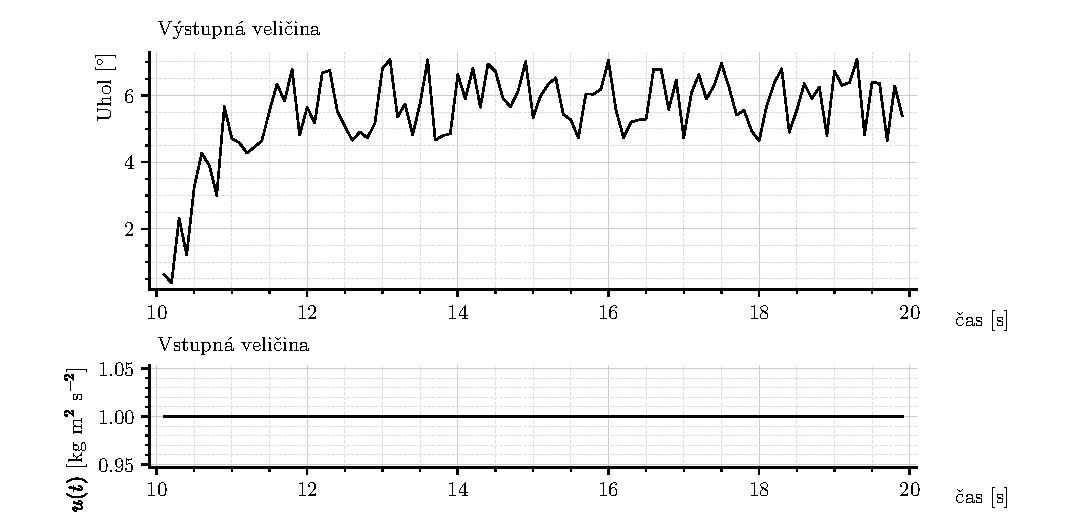
\includegraphics{MRS04_figsc_03_3.pdf}
% 	}
%
% 	\vspace{-6pt}
%
% 	\figcaption{Surové dáta - detail}
% 	\label{Surové dáta - detail}
%
% 	\vspace{-6pt}
%
% 	\end{figure}
%
% % \end{center}





% % \begin{center}
%
% 	\begin{figure}[b]
% 	\centering
%
%     \makebox[\textwidth][c]{%
% 	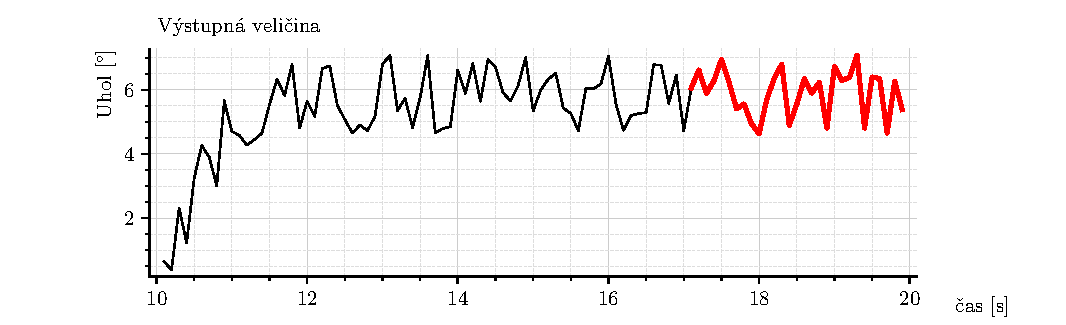
\includegraphics{MRS04_figsc_04_4.pdf}
% 	}
%
% 	\vspace{-6pt}
%
% 	\figcaption{Surové dáta - detail}
% 	\label{Surové dáta - detail2}
%
% 	\vspace{-6pt}
%
% 	\end{figure}
%
% % \end{center}





\begin{center}

	\makebox[\textwidth][c]{%
	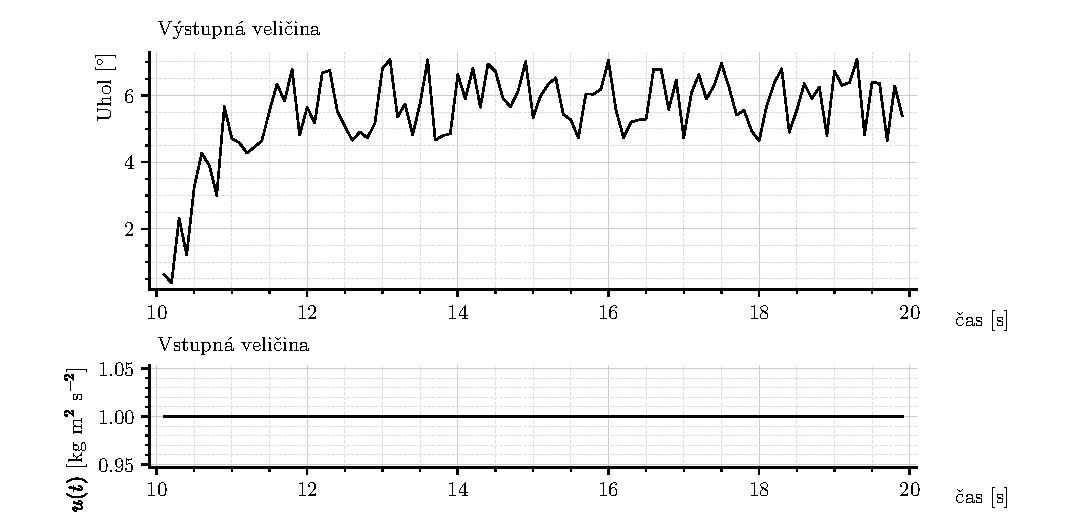
\includegraphics{MRS04_figsc_03_3.pdf}
	}

	% \vspace{-6pt}

	\figcaption{Surové dáta - detail}
	\label{Surové dáta - detail}

	% \vspace{-6pt}


	\makebox[\textwidth][c]{%
	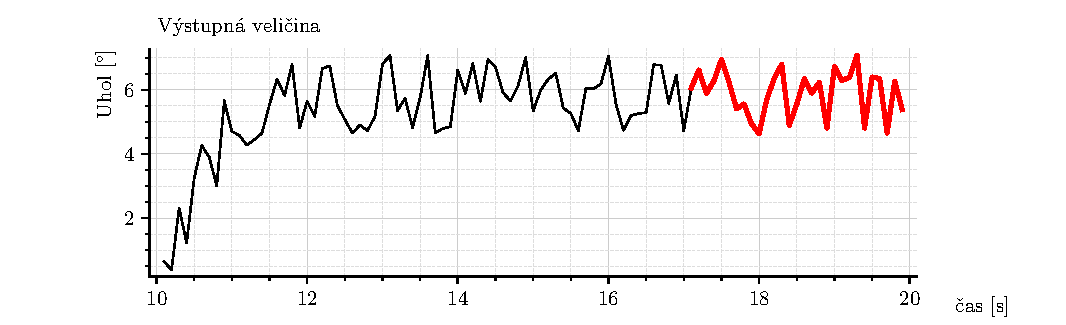
\includegraphics{MRS04_figsc_04_4.pdf}
	}

	% \vspace{-6pt}

	\figcaption{Surové dáta - detail}
	\label{Surové dáta - detail2}

	% \vspace{-6pt}

    \makebox[\textwidth][c]{%
	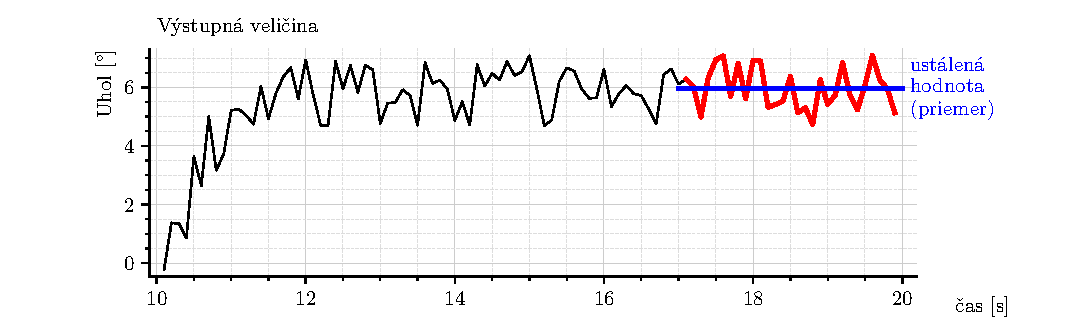
\includegraphics{MRS04_figsc_05_5.pdf}
	}

	% \vspace{-6pt}

	\figcaption{Surové dáta - detail}
	\label{Surové dáta - detail3}

	% \vspace{-6pt}

	\makebox[\textwidth][c]{%
		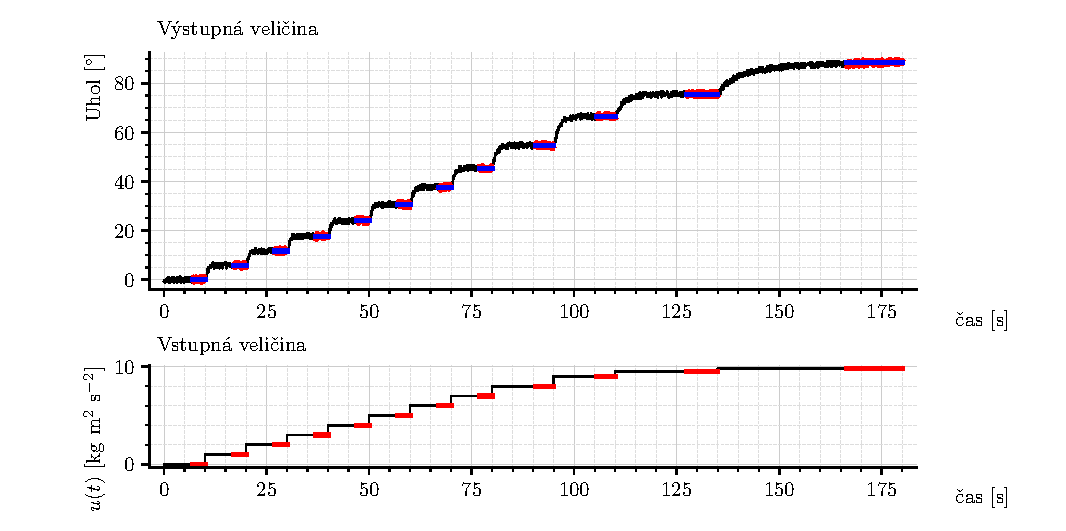
\includegraphics{MRS04_figsc_06_6.pdf}
		}

	% \vspace{-6pt}

	\figcaption{Surové dáta}
	\label{Surové dáta2}

	% \vspace{-6pt}


    \makebox[\textwidth][c]{%
	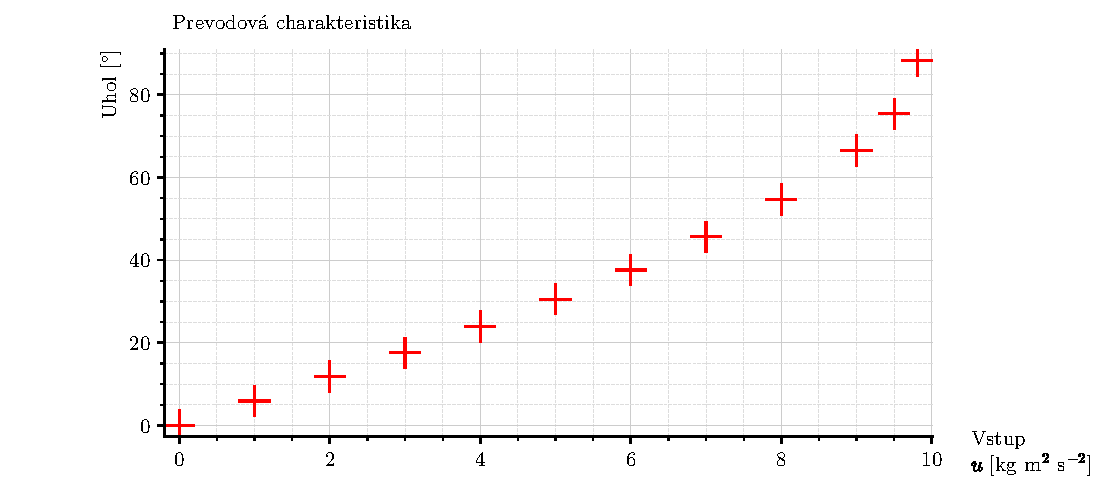
\includegraphics{MRS04_figsc_07_7.pdf}
	}

	% \vspace{-6pt}

	\figcaption{Prevodová charakteristika}
	\label{Prevodová charakteristika graf}


\end{center}





% \begin{center}
%
% 	\vspace{-6pt}
%
%     \makebox[\textwidth][c]{%
% 	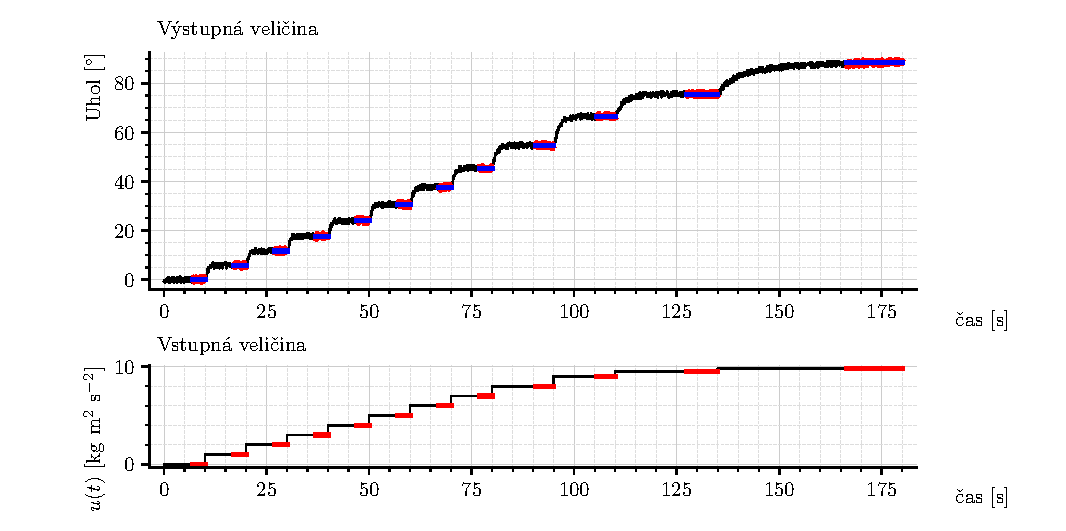
\includegraphics{MRS04_figsc_06_6.pdf}
% 	}
%
% 	\vspace{-12pt}
%
% 	\figcaption{Surové dáta}
% 	\label{Surové dáta2}
%
% 	% \vspace{-6pt}
%
% \end{center}


% \begin{center}
%
%     \makebox[\textwidth][c]{%
% 	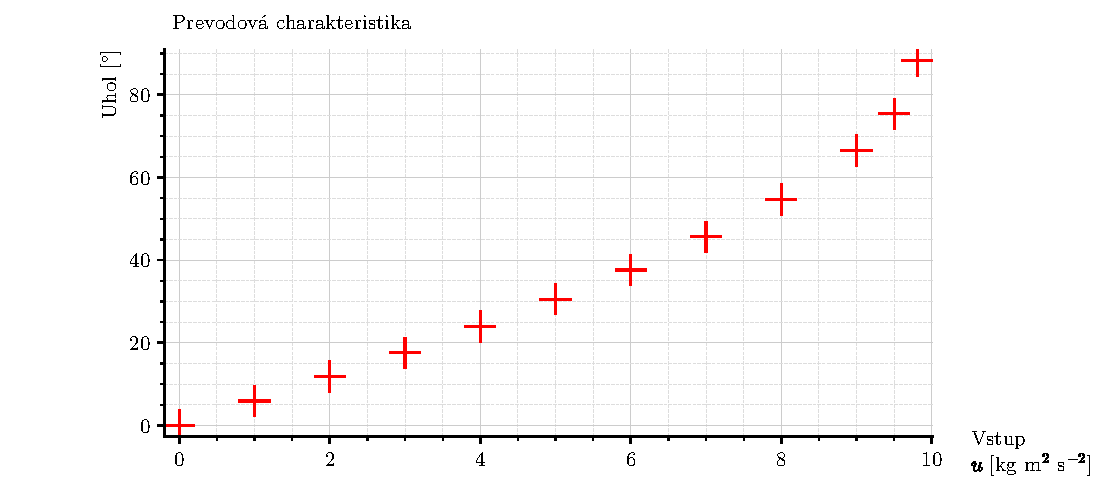
\includegraphics{MRS04_figsc_07_7.pdf}
% 	}
%
% 	\figcaption{Prevodová charakteristika}
% 	\label{Prevodová charakteristika graf}
%
% \end{center}
%





















\section{Doplnkový text: o aproximácii prevodovej charakteristiky lineárnym modelom}




\begin{itemize}[leftmargin=0pt, labelsep=4mm, itemsep=0pt]
    \color{Blue}

    \item Táto časť je len informatívna. NEBUDE predmetom záverečnej skúšky. Je tu uvedená pre náznak úplnosti a ako podnet k rozširovaniu si všeobecného prehľadu.

\end{itemize}


\noindent
Majme nameranú prevodovú charakteristiku, dáta sú v tabuľke~\ref{Prevodová charakteristika}. Prevodová charakteristika je graficky znázornená na obr.~\ref{Prevodová charakteristika graf}.



\subsection{Model}

Body prevodovej charakteristiky zodpovedajú istej vlastnosti reálneho systému (reálne existujúceho systému). Zodpovedajú závislosti výstupu systému od vstupu systému, samozrejme v ustálenom stave. Nameraných je však len niekoľko bodov. V týchto bodoch je daná vlastnosť systému známa. Čo však v prípade ak by bolo potrebné poznať danú vlastnosť mimo nameraných bodov? Teda mimo hodnôt vstupu, pre ktoré bola prevodová charakteristika nameraná.

Aj pre tieto účely je výhodné využiť model. Model reálnej vlastnosti systému. Samotnej vlastnosti systému zodpovedá nameraná závislosť (prevodová charakteristika). Aproximáciou tejto závislosti je možné získať model.

Model nech je v tomto prípade matematický vzťah, funkčná závislosť, istý predpis... Ak hodnota na vstupe modelu bude rovnaká ako hodnota na vstupe reálneho systému, potom hodnota na výstupe modelu nech je „približne rovnaká“ ako hodnota reálna. Toto nech však platí pre všetky namerané body prevodovej charakteristiky. Teda model nech sa približne zhoduje s reálnymi dátami. Ak toto platí v nameraných bodoch, potom to, zrejme, platí aj v iných bodoch. Platí to pre akúkoľvek hodnotu na vstupe modelu - že výstup modelu sa približne zhoduje s reálnym výstupom systému.



Takto všeobecne opísaný model možno skonkretizovať napríklad nasledovne: Nech modelom je polynomiálna funkcia
\begin{equation} \label{polyFcnDef}
    \hat y = \Theta_3 u^3 + \Theta_2 u^2 + \Theta_1 u + \Theta_0
\end{equation}
kde „vstup modelu“ je $u$ a „výstup modelu“ je $\hat y$. Parametrami modelu sú koeficienty (čísla) $\Theta_3$, $\Theta_2$, $\Theta_1$ a $\Theta_0$.

Mimochodom, ide o lineárny model. Parametre modelu sú v lineárnom vzťahu k~„signálom“ modelu (k~vstupom modelu).



\subsection{Jednoduché hľadanie parametrov (koeficientov) polynómu}

V tejto časti sa použije MATLAB pre nájdenie parametrov (koeficientov) polynomiálnej funkcie \eqref{polyFcnDef}. Pre tieto účely majme premennú \verb|prevodChar|, ktorej prvý stĺpec sú hodnoty vstupnej veličiny a druhý stĺpec sú hodnoty výstupnej veličiny. Teda obr.~\ref{Prevodová charakteristika graf} by sme v MATLABe nakreslili takto
\begin{lstlisting}[language=Matlab, numbers=none]
figure(1);
plot(prevodChar(:,1), prevodChar(:,2), '+r');
\end{lstlisting}




\subsubsection{Funkcia polyfit}

Funkcia \verb|polyfit| slúži vo všeobecnosti na hľadanie koeficientov polynómu (polynomiálnej funkcie) daného stupňa tak aby polynomiálna funkcia aproximovala dané dáta (napr. nameranú x-y závislosť). Kritériom pre hľadanie koeficientov je minimalizácia štvorcov (kvadrátov) odchýlok medzi nameranou hodnotou a jej aproximáciou. Presnejšie, minimalizácia sumy štvorcov odchýlok.

Použitie funkcie \verb|polyfit| v tu uvažovanom konkrétnom prípade by bolo nasledovné
\begin{lstlisting}[language=Matlab, numbers=none]
polyKoef = polyfit(prevodChar(:,1),prevodChar(:,2), 3)
\end{lstlisting}
a premenná \verb|polyKoef| obsahuje hodnoty koeficientov polynómu. Rovnica \eqref{polyFcnDef} s~nájdenými koeficientami je:
\begin{equation} \label{modelPolifitVysl}
    \hat y = 0,1111 u^3  -1,1150 u^2 + 8,9102 u  -1,1770
\end{equation}


\subsubsection{Funkcia polyval}

Pre vypočítanie hodnôt (výstupov) $\hat y$ pre požadované vstupy $u$ je možné použiť funkciu \verb|polyval|. Ak teda chceme ku každému vstupu, pre ktorý bola nameraná hodnota výstupu, vypočítať jej aproximáciu $\hat y$ podľa modelu \eqref{modelPolifitVysl}, potom stačí zavolať:
\begin{lstlisting}[language=Matlab, numbers=none]
y_hat = polyval(polyKoef, prevodChar(:,1));
\end{lstlisting}
Obrázok, na ktorom sú naraz zobrazené namerané dáta aj výstup modelu \eqref{modelPolifitVysl} možno nakresliť nasledovne:
\begin{lstlisting}[language=Matlab, numbers=none]
figure(2);
hold on;
plot(prevodChar(:,1), prevodChar(:,2), '+r')
plot(prevodChar(:,1), y_hat, '.b')
\end{lstlisting}
Samotný obrázok by bol podobný obr.~\ref{Prevodová charakteristika namer vs model}


\begin{figure}[t]
	\centering

    \makebox[\textwidth][c]{%
	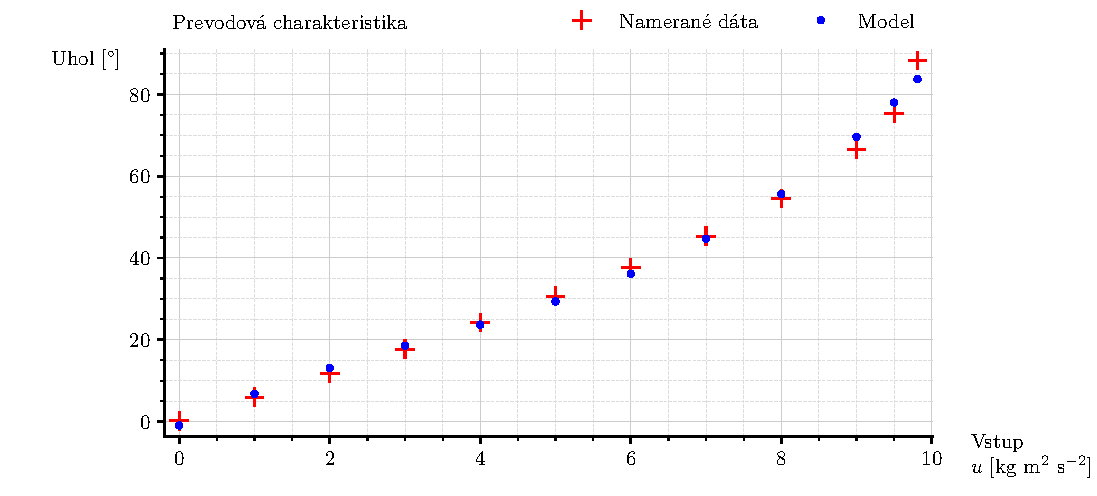
\includegraphics{MRS04_figsc_02_a_2.pdf}
	}

    \vspace{-4mm}

	\caption{Prevodová charakteristika}
	\label{Prevodová charakteristika namer vs model}

\end{figure}



\subsubsection{Používanie modelu}

Model, samozrejme, umožňuje vypočítať aproximáciu reálneho výstupu pre akúkoľvek hodnotu vstupu - nie len pre hodnoty vstupov, pre ktoré boli merané hodnoty skutočného systému. Vypočítajme výstupy modelu pre tieto vstupné hodnoty (dané vektorom):
\begin{lstlisting}[language=Matlab, numbers=none]
u_ine = [0:0.1:9.81];
\end{lstlisting}
Teda zavoláme funkciu \verb|polyval|.
\begin{lstlisting}[language=Matlab, numbers=none]
y_ine_1 = polyval(polyKoef, u_ine);
\end{lstlisting}
Nakreslime obrázok (viď obr.~\ref{Prevodová charakteristika nuine})
\begin{lstlisting}[language=Matlab, numbers=none]
figure(3);
hold on;
plot(prevodChar(:,1), prevodChar(:,2), '+r')
plot(u_ine, y_ine_1, '.b')
\end{lstlisting}


\begin{figure}[t]
	\centering

    \makebox[\textwidth][c]{%
	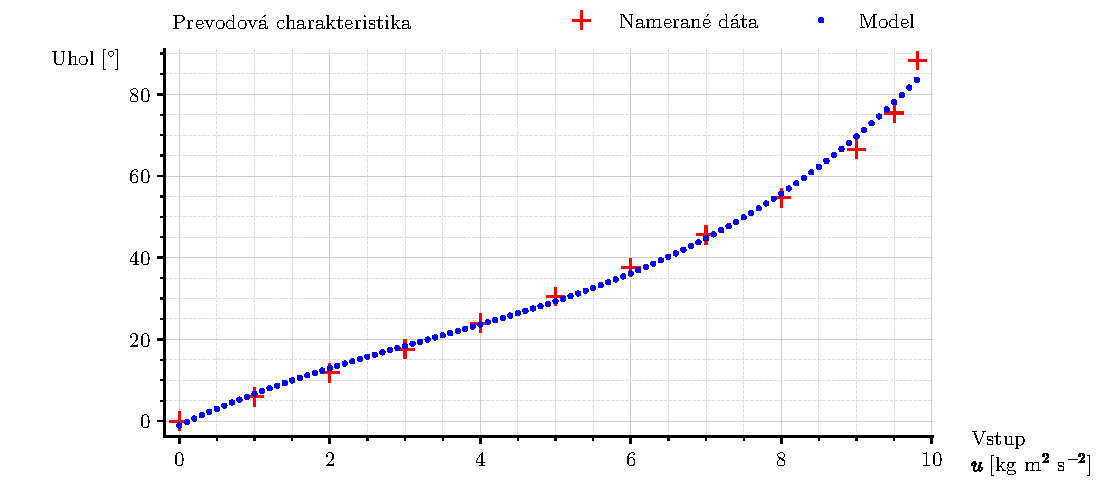
\includegraphics{MRS04_figsc_03_a_3.pdf}
	}

    \vspace{-4mm}

	\caption{Prevodová charakteristika}
	\label{Prevodová charakteristika nuine}

\end{figure}





\subsection{Čo vlastne robí funkcia polyfit}

V MATLABe funkcia \verb|polyfit| zostaví istú sústavu rovníc a následne sa použije, pre MATLAB ikonický, príkaz „backslash“: \verb|\|. Dokonca niektorí ľudia nosia na tričku nápis (niektorí nie, pretože také tričko nemajú): \verb|x = A\b;|


O tom, že funkcia \verb|polyfit| používa príkaz „backslash“, sa čitateľ môže ľahko presvedčiť otvorením súboru, v ktorom je funkcia definovaná. Stačí zadať príkaz (do Command Window):
\begin{lstlisting}[language=Matlab, numbers=none]
open polyfit
\end{lstlisting}
Otvorí sa súbor \verb|polyfit.m| a na riadku číslo 65 sa používa príkaz „backslash“.



\subsubsection{Preurčená sústava rovníc}

Tu sa pokúsime naznačiť, akú sústavu rovníc zostaví a~potom rieši funkcia \verb|polyfit| aby našla to čo hľadá - hľadá koeficienty polynómu v~zmysle istého kritéria (minimalizovať sumu štvorcov odchýlok medzi nameranými dátami a výstupom modelu).

Podobne sa dá postupovať nie len práve pri hľadaní nejakých koeficientov polynómu. Podobný postup je možné použiť pri hľadaní parametrov lineárneho modelu vo všeobecnosti. Pritom však dôkladnejšie vysvetlenie pojmu \emph{lineárny model} a~\emph{identifikácia} jeho parametrov je praďaleko nad rámec tohto textu, predmetu, a~asi aj bakalárskeho študijného programu.

Akokoľvek, aspoň náznak pre ilustráciu istotne má zmysel.


Preurčená sústava rovníc je sústava algebraických rovníc, taká, že počet rovníc je väčší ako počet neznámych. Tu by bolo možné pridať značné množstvo detailov. Na niektoré si azda čitateľ spomína zo svojho štúdia lineárnej algebry.

Ak má sústava rovníc toľko neznámych koľko rovníc, potom je riešenie jednoznačné (iba ak by nebolo).

Ak má sústava rovníc menej neznámych ako je počet rovníc, potom riešenie pri prvom intuitívnom priblížení neexistuje. Avšak sú prípady, keď je potrebné „aspoň nejako“ vyriešiť takúto sústavu rovníc. Taký prípad sa vyskytuje napríklad aj pri používaní funkcie \verb|polyfit| tak ako bola použitá vyššie.

Preurčenú sústavu rovníc je možné riešiť v zmysle tzv. \emph{metódy najmenších štvorcov}. Algebraický pohľad na vec tu vynechajme, ale aplikovanie tejto „metódy“ sa v našom prípade prejaví tak, že suma štvorcov odchýlok medzi nemeranými dátami a výstupom modelu je minimálna možná.




\bigskip

Pripomeňme, že sa zaoberáme prípadom, keď modelom je polynomiálna funkcia v~tvare
\begin{equation}
    \hat y = \Theta_3 u^3 + \Theta_2 u^2 + \Theta_1 u + \Theta_0
\end{equation}
čo je rovnica \eqref{polyFcnDef} a teda „vstup modelu“ je $u$ a „výstup modelu“ je $\hat y$. Parametrami modelu sú koeficienty (čísla) $\Theta_3$, $\Theta_2$, $\Theta_1$ a $\Theta_0$.


Ak by sme na vstup modelu priviedli hodnotu zodpovedajúcu prvému bodu prevodovej charakteristiky (súradnice bodu označme $[u_1, y_1]$) potom na výstupe modelu by bola hodnota, ktorú označme $\hat y_1$. Presnejšie napísané:
\begin{equation}
    \hat y_1 = \Theta_3 u_1^3 + \Theta_2 u_1^2 + \Theta_1 u_1 + \Theta_0
\end{equation}
Pre druhý bod prevodovej charakteristiky by to bolo
\begin{equation}
    \hat y_2 = \Theta_3 u_2^3 + \Theta_2 u_2^2 + \Theta_1 u_2 + \Theta_0
\end{equation}
atď\ldots

Samozrejme, model má v každom prípade len jednu sadu parametrov: $\Theta_3$, $\Theta_2$, $\Theta_1$ a $\Theta_0$. Tie, samozrejme, ostávajú rovnaké bez ohľadu na to aký je vstup modelu.




Model má aproximovať reálne dáta (reálnu vlastnosť systému). Odchýlky medzi modelom a dátami v jednotlivých nameraných bodoch sú:
\begin{subequations}
    \begin{align}
        e_1 &= y_1 - \hat y_1 \\
        e_2 &= y_2 - \hat y_2 \\
        e_3 &= y_3 - \hat y_3 \\
        &\vdots
    \end{align}
\end{subequations}
Odchýlky teda sú $e_1$, $e_2$, atď. Za $\hat y_i$, pre $i = 1,\ldots, N$, možno dosadiť vyššie uvedené, teda
\begin{subequations}
    \begin{align}
        e_1 &= y_1 - \Theta_3 u_1^3 + \Theta_2 u_1^2 + \Theta_1 u_1 + \Theta_0 \\
        e_2 &= y_2 - \Theta_3 u_2^3 + \Theta_2 u_2^2 + \Theta_1 u_2 + \Theta_0 \\
        e_3 &= y_3 - \Theta_3 u_3^3 + \Theta_2 u_3^2 + \Theta_1 u_3 + \Theta_0 \\
        &\vdots \\
        e_N &= y_N - \Theta_3 u_N^3 + \Theta_2 u_N^2 + \Theta_1 u_N + \Theta_0
    \end{align}
\end{subequations}

Ak by sa model presne zhodoval s dátami, potom by platilo
\begin{subequations}
    \begin{align}
        e_1 &= 0 \\
        &\vdots \\
        e_N &= 0
    \end{align}
\end{subequations}
Toto by však bol úplne ideálny prípad a dá sa tušiť, že takýto prípad nenastane.

Akokoľvek, čo sa týka číselných hodnôt $e_i$ považujme ich na chvíľku za známe, také, že sú nulové. Potom práve vznikla sústava rovníc. Ich počet je $N$. Neznáme v rovniciach sú $\Theta_3$, $\Theta_2$, $\Theta_1$ a $\Theta_0$, teda 4 neznáme. Všetko ostatné je v rovniciach známe, teda známe sú $e_i$, $y_i$ aj $u_i$. V tomto prípade, počet rovníc je väčší ako počet neznámych. To je veľmi dôležité, avšak prečo je to dôležité je ďalšia vec čo začína byť nad rámec tohto textu.

Uvedená sústava rovníc sa dá zapísať maticovo:
\begin{equation} \label{detailPreurcVseob}
    \begin{bmatrix}
        0 \\ 0 \\\vdots \\ 0
    \end{bmatrix}
    =
    \begin{bmatrix}
        y_1 \\ y_2 \\\vdots \\ y_N
    \end{bmatrix}
    -
    \begin{bmatrix}
        u_1^3 & u_1^2 & u_1 & 1 \\
        u_2^3 & u_2^2 & u_2 & 1 \\
        \vdots & \vdots & \vdots & \vdots \\
        u_N^3 & u_N^2 & u_N & 1
    \end{bmatrix}
    \begin{bmatrix}
        \Theta_3 \\ \Theta_2 \\ \Theta_1 \\ \Theta_0
    \end{bmatrix}
\end{equation}
Pre zjednodušenie zaveďme označenia:
\begin{equation}
    0 = y - H \Theta
\end{equation}
kde je snáď zrejmé čo je čo. Inak zapísané:
\begin{equation} \label{psrtem}
    H \Theta = y
\end{equation}

Toto je (pri predpoklade o vyššom počte rovníc ako je neznámych) sústava rovníc, ktorú je možné riešiť v zmysle metódy najmenších štvorcov (kvadrátov). Podrobnosti sú ďaleko praďaleko nad rámec tohto textu. Výsledkom však je, že vektor $y$ a vektor $H \Theta$ (áno je to vektor) sa „rovnajú“ v takom zmysle, že suma kvadrátov odchýlok medzi ich súradnicami je minimálna možná. Inak, a užitočnejšie, povedané, $y - H \Theta$ je vlastne $e$. Vektor $e$ obsahuje všetky odchýlky medzi modelom a nameranými dátami. Vektor $e$ sú ale aj odchýlky medzi súradnicami vektorov, o ktorých sme práve hovorili. A suma kvadrátov týchto odchýlok je minimálna! Takže aj suma odchýlok medzi modelom a dátami je minimálna!





\subsubsection{Názorná ukážka}

Zostavme teraz, v MATLABe, maticu $H$ a vektor $y$ podľa toho čo ukazuje rovnica \eqref{detailPreurcVseob}.
\begin{lstlisting}[language=Matlab, numbers=none]
H = [prevodChar(:,1).^3, prevodChar(:,1).^2, prevodChar(:,1).^1, ones(length(prevodChar(:,1)), 1)];
y = prevodChar(:,2);
\end{lstlisting}
Neznámu nazvime \verb|Theta| a riešenie preurčeného systému rovníc \eqref{psrtem} hľadajme príkazom:
\begin{lstlisting}[language=Matlab, numbers=none]
Theta = H\y
\end{lstlisting}
Výsledkom je:
\begin{lstlisting}[language=Matlab, numbers=none]
Theta =

    0.1111
   -1.1150
    8.9102
   -1.1770
\end{lstlisting}
a to sú také isté hodnoty koeficientov ako sa uvádza v rovnici \eqref{modelPolifitVysl}.





\subsubsection{Analytický pohľad}

V predchádzajúcej časti sme použili istý príkaz („backslash“) pre hľadanie riešenia preurčeného systému algebraických rovníc v zmysle metódy najmenších štvorcov. Čo presne robí tento príkaz, aby našiel riešenie, je opäť raz ďaleko nad rámec tohto textu. Ak by sme však hľadali riešenie formulovaného problému analyticky, je možné ukázať (ale nebudeme to robiť), že to vedie na nasledujúcu rovnicu
\begin{equation}
    \Theta = \left( H^\mathsf T H \right)^{-1} H^\mathsf T y
\end{equation}
Táto rovnica je známa pod názvom \emph{Gaussov vzorec}.

Pri použití tejto rovnice je potrebné urobiť inverziu istej matice - ako je zrejmé\ldots \  Práve táto inverzia matice môže byť (a v praxi veľmi často je) z~hľadiska numerických výpočtov veľmi náročnou operáciou (a napríklad aj toto rieši efektívnejšie príkaz „backslash“).

Použime tento vzorec (rovnicu) priamo v MATLABe:
\begin{lstlisting}[language=Matlab, numbers=none]
Theta_1 = inv(H'*H)*H'*y
\end{lstlisting}
Výsledkom je:
\begin{lstlisting}[language=Matlab, numbers=none]
Theta_1 =

    0.1111
   -1.1150
    8.9102
   -1.1770
\end{lstlisting}
a to sú opäť také isté hodnoty koeficientov ako sa uvádza v rovnici \eqref{modelPolifitVysl}.




\subsection{Všetko uvedené realizované v jazyku Python}


Nasledujúce je ukážkou príkazov v jazyku Python, kde sa využíva knižnica (modul) \verb|numpy|. Príkazy realizujú to isté ako bolo uvedené doposiaľ (pomocou príkazov v~MATLABe). Kreslenie obrázkov je tu vynechané\ldots



\begin{lstlisting}[language=Python,]
import numpy as np


# pouzitie funkcie polyfit (z modulu numpy)
polyKoef = np.polyfit(prevodChar[:,0],prevodChar[:,1], 3)


# funkcia polyval pouzita pre vypocet aproximacie nameranych hodnot vystupu
y_hat = np.polyval(polyKoef, prevodChar[:,0])


# vypocitanie aproximacie vystupu pre rozne vstupne hodnoty
u_ine = np.arange(0,9.81,0.1)
y_ine_1 = np.polyval(polyKoef, u_ine)


# zostavenie matice H a vektora y

H = np.hstack([
        (prevodChar[:,0].reshape(-1,1))**3,
        (prevodChar[:,0].reshape(-1,1))**2,
        prevodChar[:,0].reshape(-1,1),
        np.ones([prevodChar[:,0].shape[0],1]),
        ])

y = prevodChar[:,1].reshape(-1,1)


# Riesenie preurceneho systemu rovnic v zmysle metody najmensich stvorcov
Theta = np.linalg.lstsq(H, y, rcond=None)[0]

# Pouzitie Gaussovho vzorca
Theta_1 = np.matmul(np.matmul(np.linalg.inv(np.matmul(H.T, H)), H.T), y)

\end{lstlisting}






\section{O meraní prechodovej charakteristiky}


% \begin{itemize}[leftmargin=0pt, labelsep=4mm, itemsep=0pt]
%     \color{Gray}

%     \item Ponechajme si tu názov časti, že „O meraní\ldots“ aj keď v dobe rúškovej sa nerealizuje meranie, len simulácia\ldots

% \end{itemize}


\subsection{Úvod}

Nasledujúci text má za cieľ inšpirovať čitateľa tak, aby získal lepšiu predstavu o~tom ako zrealizovať zmysluplné meranie prechodových charakteristík (aj keď v tomto prípade sa čitateľ bude zaoberať len simuláciami). V tomto prípade totiž nie je úlohou len samotné získanie prechodovej charakteristiky. Potrebný je tiež rozbor problému z hľadiska daného reálneho (simulovaného) systému (ktorého vlastnosti skúmame). Preto je v prvom rade potrebné vysvetlenie pojmov používaných pri opise dynamického systému.



Pripomeňme, že v tomto bode máme dostupnú istú informáciu o predmetnom skúmanom systéme. Je ňou prevodová charakteristika - viď obr.~\ref{Prevodová charakteristika graf}.


Samotná prevodová charakteristika vystihuje tzv. statické vlastnosti systému. Vlastnosti systému v ustálenom stave. Celkom konkrétne je možné z prevodovej charakteristiky získať statické zosilnenie systému.

Prevodová charakteristika na obr.~\ref{Prevodová charakteristika graf} ukazuje, že zosilnenie systému pri nižších hodnotách vstupného signálu je iné ako zosilnenie pri vyšších hodnotách vstupného signálu. Využime skutočnosť, že v tomto prípade máme dostupný model prevodovej charakteristiky (nie je nevyhnutné mať takýto model). Modelom je polynomiálna funkcia, konkrétne:
\begin{equation} \label{modelPolifitVysl2}
    \hat y = 0,1111 u^3  -1,1150 u^2 + 8,9102 u  -1,1770
\end{equation}
Použime tento model pre vypočítanie výstupov (odhadov výstupov) systému v týchto hodnotách vstupného signálu:
\begin{lstlisting}[language=Matlab, numbers=none]
u_ine = [0:0.1:9.81];
\end{lstlisting}
Získame nasledujúci obrázok (pozri obr.~\ref{Prevodová charakteristika graf2}).



\begin{figure}[t]
	\centering

    \makebox[\textwidth][c]{%
	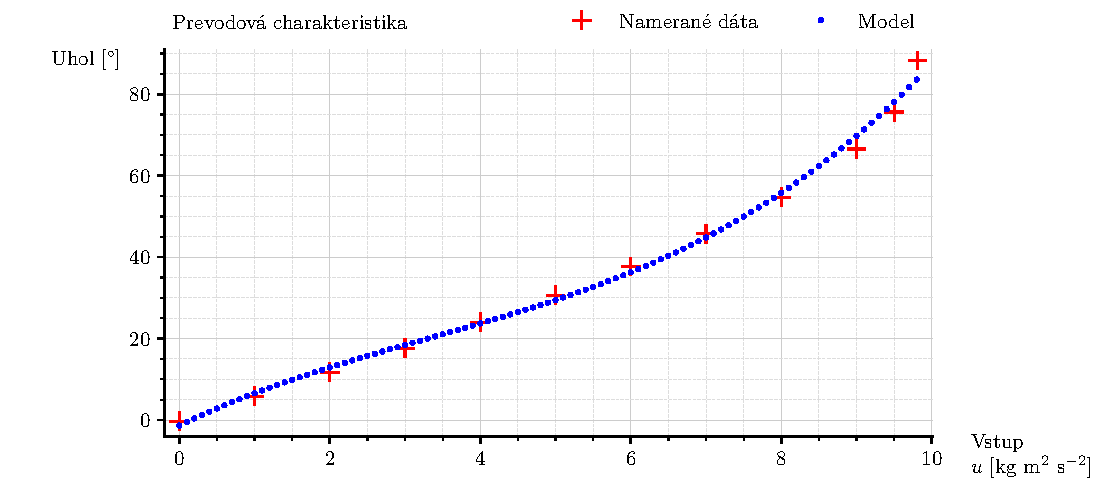
\includegraphics{MRS04_figsc_03_a_666.pdf}
	}

    \vspace{-4mm}

	\caption{}
	\label{Prevodová charakteristika graf2}

\end{figure}


\begin{figure}[t]
	\centering

    \makebox[\textwidth][c]{%
	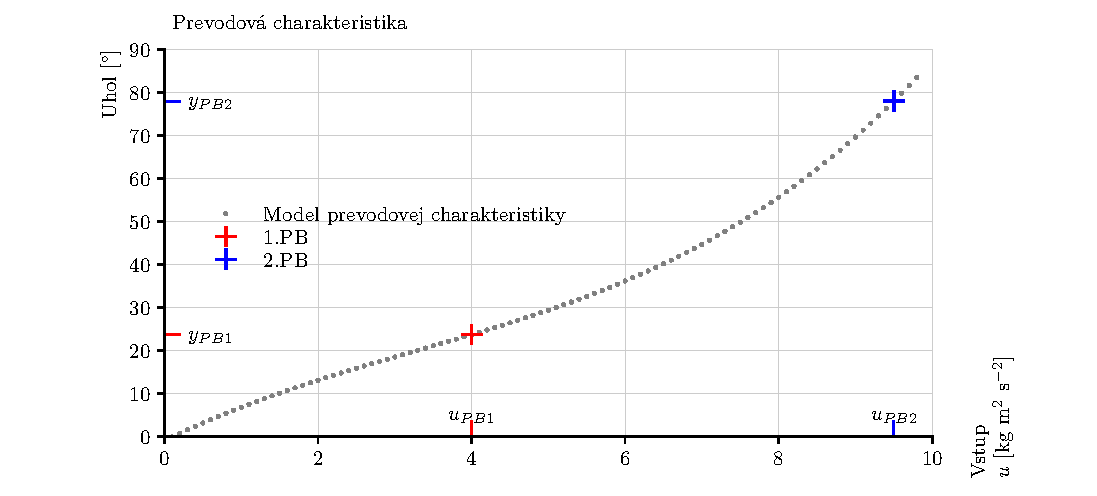
\includegraphics{MRS04_PCH_figsc_04_0.pdf}
	}

    \vspace{-4mm}

	\caption{}
	\label{Prevodová charakteristika graf4}

\end{figure}






\subsection{Stručné vysvetlenie pojmov}

Hlavnou úlohou v tomto texte je získať prechodové charakteristiky predmetného systému (laboratórny systém) v rôznych pracovných bodoch. Pracovné body nech sú zvolené s prihliadnutím na prevodovú charakteristiku systému. V prvom rade, čo je to \emph{pracovný bod}?


\bigskip


Pracovný bod je definovaný ustálenou hodnotou vstupného signálu, ku ktorej (jednoznačne) prislúcha ustálená hodnota výstupného signálu. Dvojica hodnôt, hodnota na vstupe a hodnota na výstupe, tvorí pracovný bod.

Ak je daná ustálená hodnota vstupného signálu, potom je možné pomocou prevodovej charakteristiky nájsť prislúchajúcu ustálenú hodnotu výstupného signálu.

Pojem pracovný bod na seba viaže aj pojem \emph{okolie pracovného bodu}. V okolí pracovného bodu sú vlastnosti systému relatívne rovnaké ako v pracovnom bode. Z hľadiska statických vlastností systému to znamená, že v okolí pracovného bodu sa sklon prevodovej charakteristiky relatívne nemení. Inými slovami, statické zosilnenie systému sa nemení. Rovnako aj dynamické vlastnosti systému sú v okolí pracovného bodu relatívne nemenné - časové konštanty systému sa nemenia.

V dvoch rôznych pracovných bodoch môže mať reálny systém napríklad rozdielne statické zosilnenie, teda statické vlastnosti. Statické zosilnenie systému v pracovnom bode je možné určiť na základe prevodovej charakteristiky. Je dané sklonom prevodovej charakteristiky v okolí pracovného bodu.

Prípadný rozdiel v statických vlastnostiach v rôznych pracovných bodoch však nehovorí nič o prípadnom rozdiele dynamických vlastnostiach systému. Dynamické vlastnosti je možné vyhodnocovať na základe prechodovej charakteristiky.

\emph{Prechodová charakteristika} je odozva systému na jednotkový skok.

Pod pojmom \emph{jednotkový skok} sa rozumie skoková zmena signálu (vstupného) a veľkosť tejto zmeny je jednotková. Je jednotková zmysle, že akúkoľvek veľkosť skokovej zmeny má zmysel (prípadne) vyjadriť ako násobok jednotkovej skokovej zmeny. Prirodzene sa predpokladá, že jednotková zmena je taká, že nespôsobí, že systém sa dostane mimo okolia pracovného bodu.



\subsection{Voľba pracovných bodov}



Pracovné body nech sú zvolené s prihliadnutím na prevodovú charakteristiku systému. Ako teda prihliadnuť? Ako už bolo uvedené, z prevodovej charakteristiky je zrejmé, že istá vlastnosť systému je iná pri nízkych hodnotách vstupného signálu a iná pri vysokých hodnotách. Tou vlastnosťou je statické zosilnenie. Iné než tzv. statické vlastnosti systému z prevodovej charakteristiky nie je možné vyčítať. Otázkou teda je či sú aj iné vlastnosti systému rozdielne pri rôznych hodnotách vstupného signálu.


Zvoľme preto dva pracovné body - jeden nech reprezentuje nízku hodnotu vstupného signálu a druhý vysokú. Zvolené pracovné body sú uvedené v tabuľke~\ref{Zvolené pracovné body}.


\begin{table}[!ht]
    \centering
	\catcode`\-=12

    \caption{Zvolené pracovné body}
    \label{Zvolené pracovné body}

    \begin{tabular}{ccc}
        \toprule
        PB & hodnota & jednotky \\
        \midrule
        1. & $4$ & [kg m$^2$ s$^{-2}$] \\
        2. & $9,5$ & [kg m$^2$ s$^{-2}$] \\
        \bottomrule
    \end{tabular}

\end{table}


Na základe nameraných bodov prevodovej charakteristiky by sme mohli k~zvoleným ustáleným vstupným hodnotám priradiť výstupné hodnoty:

\noindent
\begin{tabular}{@{}l l}
    1.PB: & $y=24,2$ [°] \\
    2.PB: & $y=75,5$ [°]
\end{tabular}


\bigskip

Pracujme však s aproximáciou prevodovej charakteristiky, teda s jej modelom. Model nám umožní získať aj také informácie, ktoré neboli reálne namerané.

Pre $u = 4$ [kg m$^2$ s$^{-2}$] podľa modelu prevodovej charakteristiky prislúcha hodnota ustáleného výstupu:
\begin{equation}
    \hat y_{PB1} = 0,1111\ u_{PB1}^3  -1,1150\ u_{PB1}^2 + 8,9102\ u_{PB1}  -1,1770
\end{equation}
kde ak $u_{PB1} = 4$ [kg m$^2$ s$^{-2}$], potom $\hat y_{PB1} = 23,73$ [°]. Podobne pre $u = 9,5$ [kg m$^2$ s$^{-2}$] podľa modelu prevodovej charakteristiky prislúcha hodnota ustáleného výstupu $\hat y_{PB2} = 78,06$ [°]. Znázornime pracovné body - viď obr.~\ref{Prevodová charakteristika graf4}.


Ďalej je, samozrejme, potrebné vhodne zvoliť okolie pracovného bodu (pre každý pracovný bod). V podstate je potrebné voliť pracovný bod a prislúchajúce okolie pracovného bodu naraz. Len tu sme to pre lepšiu názornosť oddelili.

Pripomeňme, že v okolí pracovného bodu sa očakáva, že vlastnosti systému sú relatívne nemenné. Na základe prevodovej charakteristiky možno posúdiť statické vlastnosti systému. Na základe toho, pre 1. pracovný bod (PB1) zvoľme okolie $u = 4 \pm 0,8$ [kg m$^2$ s$^{-2}$]. Pre PB2 zvoľme $u = 9,5 \pm 0,25$ [kg m$^2$ s$^{-2}$]. Znázornime pracovné body a ich okolia - viď obr.~\ref{Prevodová charakteristika graf5}. Na obrázku~\ref{Prevodová charakteristika graf5} sú tiež vyznačené hranice okolia pracovného bodu, napr. $u_{PB1_l}$ ako dolná hranica okolia pracovného bodu a~$u_{PB1_h}$ ako horná hranica. K tomu zodpovedajúce hodnoty výstupnej veličiny, hodnoty $y_{PB1_l}$ a~$y_{PB1_h}$ sú taktiež vyznačené. Obdobne aj pre druhý pracovný bod.


\begin{figure}[t]
	\centering

    \makebox[\textwidth][c]{%
	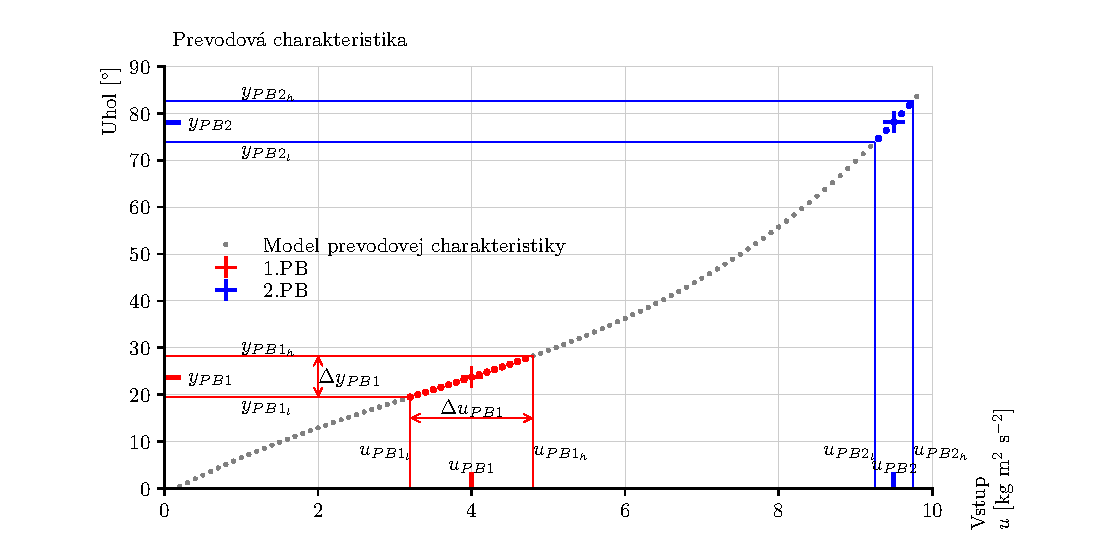
\includegraphics{MRS04_PCH_figsc_05_0.pdf}
	}

    \vspace{-4mm}

	\caption{}
	\label{Prevodová charakteristika graf5}

\end{figure}

Ďalej je v tomto prípade potrebné uvážiť veľkosť skokovej zmeny, ktorú budeme používať ako jednotkovú. Vzhľadom na okolnosti nie je dôvod, aby jednotkovou veľkosťou nebola hodnota definujúca okolie pracovného bodu. Spĺňa sa tak požiadavka, že jednotkový skok nespôsobí, že systém sa dostane mimo okolia pracovného bodu (bude na hrane, ale nie mimo). Preto pre PB1 nech je jednotková veľkosť skokovej zmeny rovná hodnote $u_{s1} = 0,8$ [kg m$^2$ s$^{-2}$] a pre PB2 nech je jednotková veľkosť skoku rovná hodnote $u_{s2} = 0,25$ [kg m$^2$ s$^{-2}$].


\subsection{Zrealizovanie merania prechodovej charakteristiky}


Aby bolo možné vykonať jednotkový skok (skokovú zmenu vstupného signálu systému s jednotkovou veľkosťou) v okolí pracovného bodu najskôr je potrebné dostať systém do pracovného bodu. Ak bude hodnota vstupného signálu $u_{PB}$, a necháme ju tak nejaký čas, potom očakávame, na základe prevodovej charakteristiky, že výstup systému sa ustáli na hodnote $y_{PB}$. Systém bude v pracovnom bode. Potom je možné skokovo zvýšiť hodnotu vstupného signálu o hodnotu $u_{s}$. Tým sa zrealizuje jednotkový skok v okolí pracovného bodu. Simulácia uvedeného je na obr.~\ref{graf6}.



\begin{figure}[t]
	\centering

    \makebox[\textwidth][c]{%
	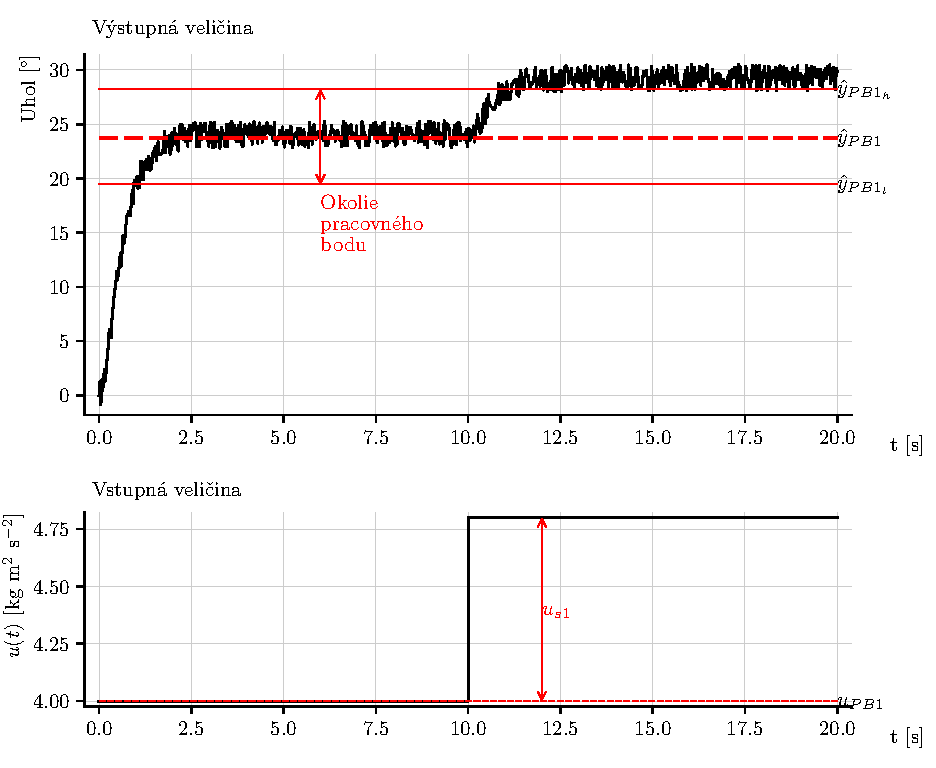
\includegraphics{MRS04_PCH_figsc_06_0.pdf}
	}

    \vspace{-4mm}

	\caption{}
	\label{graf6}

    \vspace{-4mm}

\end{figure}

Veľkosť skokovej zmeny vstupného signálu je na obrázku~\ref{graf6} označená ako $u_{s1}$. V~tomto prípade, vzhľadom na zvolené okolie pracovného bodu, je $u_{s1} = 0,8$.

Jednotkový skok nastal v čase $t=10$ [s]. Pred týmto časom sa systém dostával do pracovného bodu. Od času $t=10$ [s] až pokým sa výstupná veličina systému opäť neustálila prebieha prechodový dej, to je prechodová charakteristika (keďže na vstupe bol jednotkový skok).



\begin{figure}[t]
	\centering

    \makebox[\textwidth][c]{%
	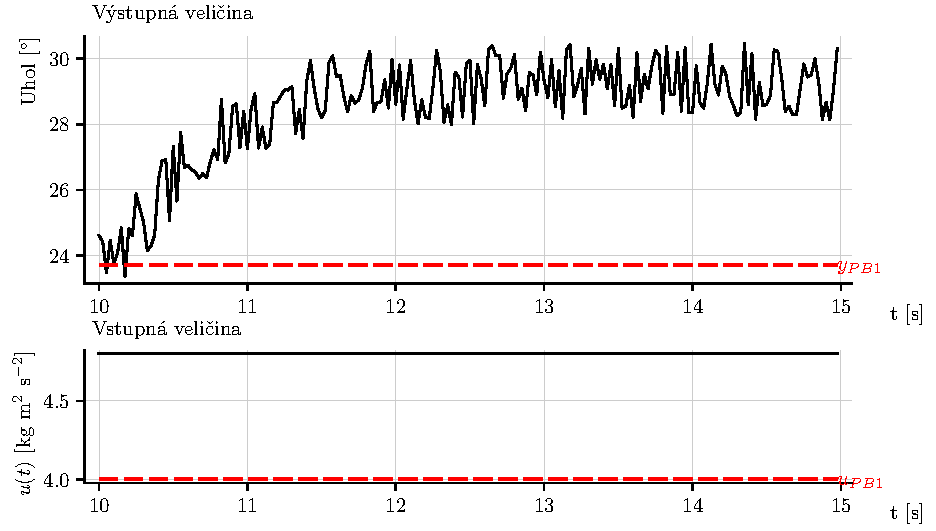
\includegraphics{MRS04_PCH_figsc_07_0.pdf}
	}

    \vspace{-4mm}

	\caption{}
	\label{graf7}

    \vspace{-4mm}

\end{figure}


\begin{figure}[!hb]
	\centering

    \makebox[\textwidth][c]{%
	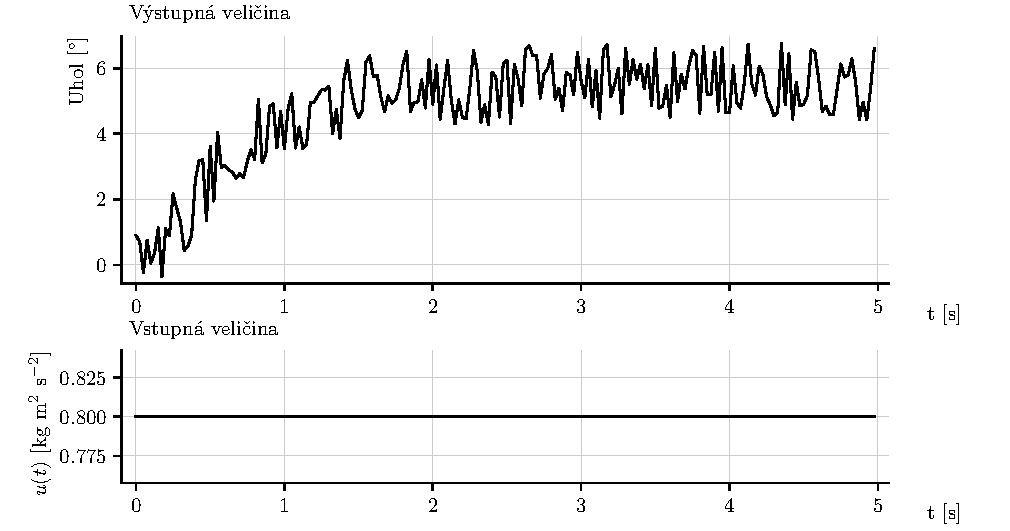
\includegraphics{MRS04_PCH_figsc_08_0.pdf}
	}

    \vspace{-4mm}

	\caption{}
	\label{graf8}

\end{figure}









\subsection{Spracovanie nameraného}


Pred jednotkovým skokom sme očakávali, že výstupná veličina sa ustáli na hodnote $y_{PB}$. Podľa modelu prevodovej charakteristiky to pre tento pracovný bod je hodnota $\hat y_{PB1} = 23,73$ [°]


Priemerná hodnota výstupnej veličiny počas doby 5 sekúnd pred jednotkovým skokom je $24,04$ [°]. Odchýlka priemernej hodnoty, okolo ktorej sa systém ustálil v~pracovnom bode, od očakávanej hodnoty podľa modelu prevodovej charakteristiky je približne 1 \%. To je samozrejme prijateľná odchýlka. Ďalej teda môžeme považovať hodnotu $\hat y_{PB1}$ podľa modelu prevodovej charakteristiky za hodnotu, na ktorej bola ustálená výstupná veličina pred skokovou zmenou vstupného signálu.

Po ukončení prechodového deja sa podľa modelu prevodovej charakteristiky očakáva, že výstupná veličina sa ustáli na hodnote $\hat y_{PB1_h} = 28,19$ [°]

Už z obr.~\ref{graf6} je zrejmé, že v skutočnosti sa výstupná veličina ustáli na o niečo vyššej hodnote. Presnejšie, ak uvažujeme časový úsek po jednotkovom skoku, na ktorom je už výstupná veličina ustálená, nech je to úsek 2,5 až 5 sekúnd po jednotkovom skoku, tak na tomto úseku je priemerná hodnota výstupnej veličiny $29,2$ [°].



Ak pri hodnote $y_{PB1}$ bol rozdiel medzi očakávaným (podľa modelu prevodovej charakteristiky) a nameraným priam zanedbateľný, pri hodnote $y_{PB1_h}$ to už nie je také jednoznačné. Nie je jednoznačné, že rozdiel je zanedbateľný. Tento problém však súvisí s meraním prevodovej charakteristiky a následnou voľbou modelu prevodovej charakteristiky, ktorý sme sa tu rozhodli používať pri odhadovaní očakávaných hodnôt $y_{PB1}$ a $y_{PB1_h}$. Ak sme sa raz rozhodli používať daný model prevodovej charakteristiky, potom s prípadnými odchýlkami, ktoré zjavne nie sú omyly, je potrebné počítať.

Týmto sme chceli povedať, že napriek tomu, že čo sa očakávaných hodnôt týka, po jednotkovom skoku výstupná veličina opustila očakávané okolie pracovného bodu. Avšak je to len očakávané, odhadované okolie (na základe modelu prevodovej charakteristiky). Odchýlky od „reálnych“ hodnôt sú prijateľné a teda môžeme pokračovať bez nutnosti prehodnotiť voľbu okolia pracovného bodu.







\subsubsection{„Vystrihnutie“ prechodovej charakteristiky}

Vyberme z dát na obr.~\ref{graf6} len tú časť, ktorá zodpovedá prechodovej charakteristike, teda dáta od času 10 až po ustálenie (nech je to čas 15). Výsledkom je obr.~\ref{graf7}.





\subsubsection{„Posunutie“ prechodovej charakteristiky}



Pre potreby ďalšej práce s prechodovou charaketristikou je zvyčajne výhodné posunúť namerané dáta tak aby začiatok prechodovej charakteristiky bol v bode (0,0), to znameá, že PCH začína v  čase 0 a hodnota výstupnej veličiny v začiatku je tiež nula (aspoň filozoficky).


Konkrétne: od získaného priebehu výstupnej veličiny je potrebné odčítať hodnotu $y_{PB}$, pretože tak sa začiatok posunie v smere osi y do nuly (filozoficky... teraz nám to asi bude kaziť šum). Rovnako priebeh vstupnej veličiny je potrebné posunúť v~smere osi o hodnotu $u_{PB}$. Samozrejme, od časového vektora je potrebné odčítať čas, v~ktorom nastal jednotkový skok. Výsledok je na obr.~\ref{graf8}.










\subsection{Poznámky k odčítavaniu hodnôt z grafu prechodovej charakteristiky}



\subsubsection{Nameraná prechodová charakteristika}

Z predchádzajúceho je dostupná nameraná a spracovaná prechodová charakteristika (PCH) predmetného systému. Ide o prechodovú charakteristiku v prvom pracovnom bode. Je zobrazená na obr.~\ref{graf8}.



Ďalej sú dostupné informácie o pracovnom bode, v ktorom bola PCH meraná. Hodnota vstupného signálu v pracovnom bode je $u = 4$ [kg m$^2$ s$^{-2}$] a uvažuje sa okolie pracovného bodu $u = 4 \pm 0,8$ [kg m$^2$ s$^{-2}$].

Je dostupný podel prevodovej charakteristiky a teda je možné odhadnúť hodnotu výstupnej veličiny v pracovnom bode, teda
\begin{equation}
    \hat y_{PB1} = 0,1111\ u_{PB1}^3  -1,1150\ u_{PB1}^2 + 8,9102\ u_{PB1}  -1,1770
\end{equation}
kde $u_{PB1} = 4$ [kg m$^2$ s$^{-2}$] a teda $\hat y_{PB1} = 23,73$ [°]. Rovnako je možné vypočítať hodnotu výstupného signálu pre, nazvime to, hornú hranicu okolia pracovného bodu, to znamená pre hodnotu na vstupe $u_{PB1_h} = 4 + 0,8$ [kg m$^2$ s$^{-2}$]. Tejto zodpovedá hodnota $\hat y_{PB1_h} = 28.19$ [°].

Keďže prechodová charakteristika na obr.~\ref{graf8} je posunutá do nuly, teda od skutočných hodnôt sú odčítané hodnoty v pracovnom bode, tak urobme túto úpravu aj pre práve vypočítané hodnoty, teda
\begin{align}
    \Delta u_{PB1} &= u_{PB1_h} - u_{PB1} = 0,8 \\
    \Delta \hat y_{PB1} &= \hat y_{PB1_h} -  \hat y_{PB1} = 4,52
\end{align}




\subsubsection{Statické zosilnenie $K$}

Zistime statické zosilnenie systému v okolí uvažovaného pracovného bodu. Potrebujeme hodnotu, na ktorej sa ustálila výstupná veličina po prechodovom deji. Z grafu PCH uvažujme, že výstupná veličina je už ustálená po čase $t=3$ [s] (dajme tomu teraz takto). Priemerná hodnota výstupnej veličiny po tomto čase je $\Delta y = 5.52$ [°].

Teda, po uskutočnení jednotkového skoku v okolí pracovného bodu sa výstupná veličina zmenila o $\Delta y$ [°]. Zmena na vstupe $\Delta u$ bola, samozrejme, práve jednotková (pretože jednotkový skok). V tomto prípade má jednotkový skok veľkosť okolia pracovného bodu  $\Delta u = 0,8$ [kg m$^2$ s$^{-2}$].

Statické zosilnenie systému, na základe prechodovej charakteristiky, označme $K$, je $K = \frac{\Delta y}{\Delta u}$, číselne
\begin{equation}
     K = 6,9 \text{[°/(kg m$^2$ s$^{-2}$)]}
\end{equation}
Uvedené možno znázorniť aj do grafu - viď obr.~\ref{graf20}


\begin{figure}[t]
	\centering

    \makebox[\textwidth][c]{%
	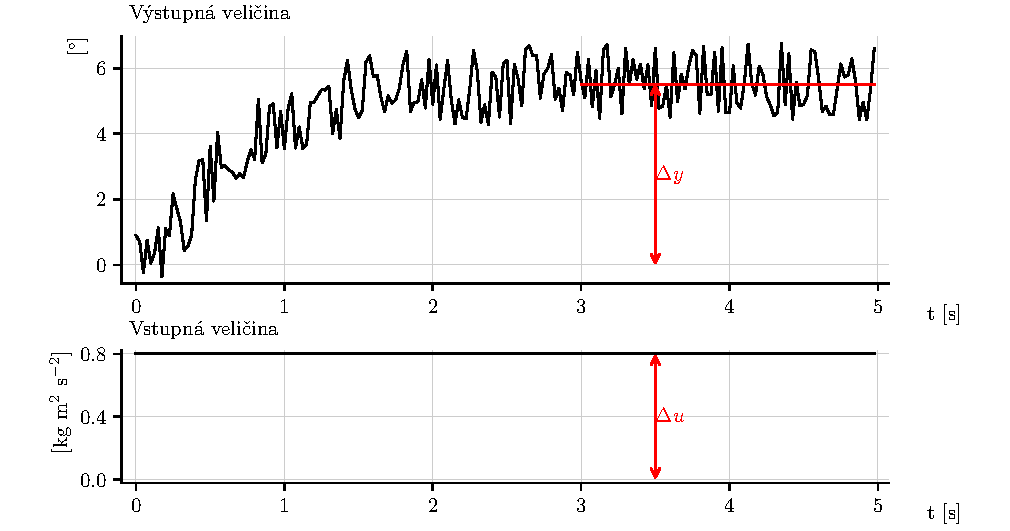
\includegraphics{MRS04_PCH_figsc_10_02_0.pdf}
	}

    \vspace{-4mm}

	\caption{}
	\label{graf20}

\end{figure}



Statické zosilnenie systému je, samozrejme, možné zistiť aj pomocou prevodovej charakteristiky. V skutočnosti, všetko potrebné už máme k dispozícii.

Mimochodom, ak by sme neboli leniví, tak nájdeme dotyčnicu v pracovnom bode, a jej smernica (sklon) by mala byť statické zosilnenie. To by bol formálne korektný postup.

My však leniví sme, preto: hľadáme sklon prevodovej charakteristiky v okolí pracovného bodu. Z praktického hľadiska, nech je sklon daný pracovným bodom a bodom ohraničujúcim okolie pracovného bodu zhora. Formálne $\text{sklon} = \frac{\Delta y}{\Delta u}$ kde $\Delta y = \hat y_{PB_h} - \hat y_{PB}$ a~$\Delta u = u_{PB_h} - u_{PB}$. To je, samozrejme, to isté ako vyplynulo z~využitia prechodovej charakteristiky vyššie. Tu však číselné hodnoty nie sú odčítané z~prechodovej charakteristiky ale z~modelu prevodovej charakteristiky. Konkrétne čísla:
\begin{equation}
    \text{sklon} = \frac{\hat y_{PB_h} - \hat y_{PB}}{u_{PB_h} - u_{PB}} = \frac{4,52}{0,8} = 5.65
\end{equation}
Odchýlka od statického zosilnenia určeného z prechodovej charakteristiky je $-1,25$ [°], t.j. $18,10$ [\%] (tá je samozrejme daná aj tým, že používame model prevodovej charakteristiky, keďže konkrétne potrebné hodnoty v rámci nameranej prevodovej charakteristiky nie sú dostupné).






\subsubsection[Časová konštanta $T$ pre lineárny dynamický systém 1. rádu]{Časová konštanta $T$ pre lineárny dynamický systém 1. rádu}


Ďalej je možné nájsť model, ktorý má vystihovať dynamiku (dynamické vlastnosti) reálneho systému. Modelom nech je lineárny dynamický systém.

Kvalifikovaný odhad založený na grafickom znázornení predmetnej prechodovej charakteristiky vedie k možnosti, že modelom systému môže byť dynamický systém 1. rádu. Tento je možné zapísať v tvare prenosovej funkcie
\begin{equation}
    G(s) = \frac{y(s)}{u(s)} = \frac{K}{Ts+1}
\end{equation}
kde $K$ je možné interpretovať ako statické zosilnenie systému a $T$ je časová konštanta.

Časovú konštantu je možné nájsť na základe prechodovej charakteristiky. Je to čas od začiatku prechodovej charakteristiky (od času jednotkového skoku), v ktorom výstupná veličina dosiahla približne 63 \% zo svojej ustálenej hodnoty.

Prečo práve 63 \%? Odpoveď sa ponecháva na čitateľa.

100 \% z ustálenej hodnoty na nasledujúcom obrázku~\ref{graf30} je samozrejme hodnota $\Delta y$. Potom 63 \% je hodnota $\Delta y_{63} =  3,48$ [°]



\begin{figure}[t]
	\centering

    \makebox[\textwidth][c]{%
	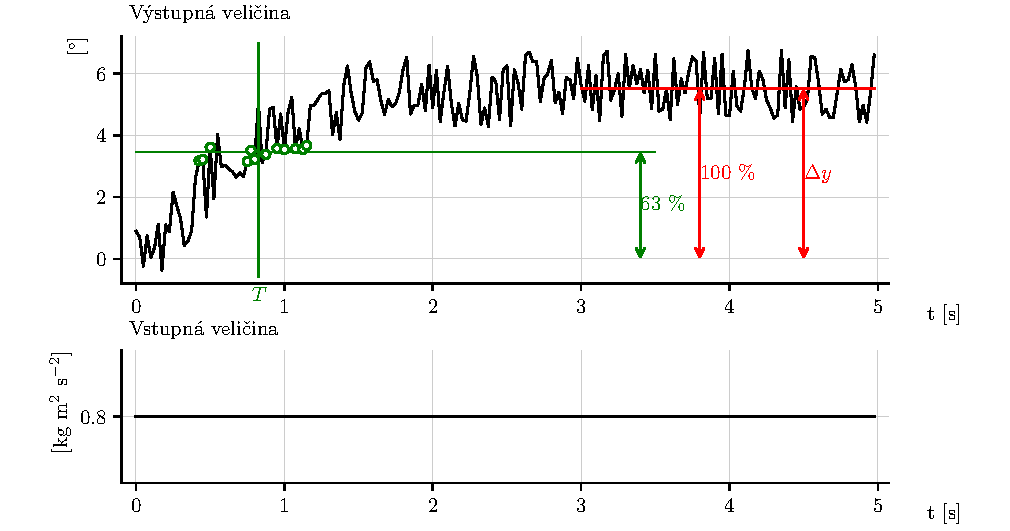
\includegraphics{MRS04_PCH_figsc_10_03_0.pdf}
	}

    \vspace{-4mm}

	\caption{}
	\label{graf30}

\end{figure}

Hodnotu $T$ teraz možno hľadať „od oka“, doslova pomocou grafu PCH, prípadne „od oka“, ale trošku inak - napr: Nájdime hodnoty výstupnej veličiny, ktoré sú v~pásme (volajme ho „od oka“) $\pm ? \%$ v okolí hodnoty $\Delta y_{63}$. Presnejšie, nájdime časy tých vzoriek, ktoré sú v~tom pásme. Nájdené body v~pásme „od oka“ okolo hodnoty $\Delta y_{63}$ sú na obr.~\ref{graf30} vyznačené ako malé zelené kružnice. Priemer z nájdených časov je
\begin{equation}
    T =  0,81 \text{[s]}
\end{equation}
A táto hodnota môže byť celkom dobre „od oka“ odčítaná časová konštanta. Všetko uvedené je nakreslené na obr.~\ref{graf30}.






\subsubsection{Verifikácia identifikovaného dynamického modelu}


V predchádzajúcom boli na základe prechodovej charakteristiky určené parametre lineárneho dynamického systému, ktorý má byť modelom skutočného systému. Tento model je možné vyjadriť v tvare prenosovej funkcie
\begin{equation}
    \frac{y(s)}{u(s)} = \frac{K}{Ts+1}
\end{equation}



Pre verifikáciu modelu je možné využiť grafické porovnanie prechodovej charakteristiky modelu a skutočnej prechodovej charakteristiky. Pre získanie PCH modelu využime numerickú simuláciu. Daná prenosová funkcia zodpovedá diferenciálnej rovnici v tvare
\begin{align}
    T \dot y(t) + y(t) &= K u(t) \\
    T \dot y(t) &= - y(t) + K u(t) \\
    \dot y(t) &= - \frac{1}{T} y(t) + \frac{K}{T} u(t)
\end{align}
Vstupný signál zvoľme rovnaký ako je veľkosť $\Delta u$. Tak zabezpečíme zodpovedajúcu veľkosť jednotkového skoku, ktorý je použitý v numerickej simulácii pre získanie PCH.

Do spoločného obrázka nakreslime nameranú PCH a PCH modelu systému - viď obr.~\ref{graf40}

\begin{figure}[t]
	\centering

    \makebox[\textwidth][c]{%
	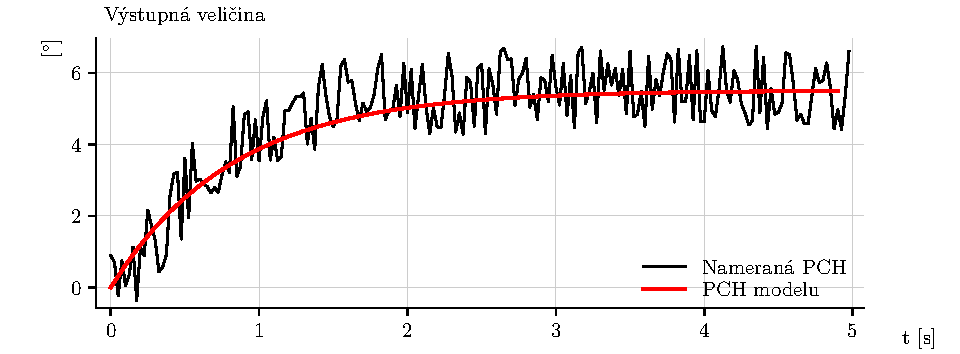
\includegraphics{MRS04_PCH_figsc_10_04_0.pdf}
	}

    \vspace{-4mm}

	\caption{}
	\label{graf40}

\end{figure}

Týmto (aspoň pre naše potreby) možno model považovať za verifikovaný - znamená to, že daný model je schopný vystihnúť vlastnosti skutočného systému a že je možné na základe dostupných informácií (prechodová charakteristika) nájsť parametre modelu.





























\section{Otázky a úlohy}

\begin{enumerate}[leftmargin=0pt, labelsep=3mm, itemsep=0pt]

    
    \item Vysvetlite pojem \emph{prevodová charakteristika systému}.

        \item Ako sa nazýva vzájomná závislosť medzi ustálenými hodnotami výstupného signálu systému a ustálenými hodnotami vstupného signálu?

        \item Čo určuje sklon prevodovej charakteristiky?


        \item Vysvetlite pojem \emph{prechodová charakteristika systému}.

        \item Ako sa nazýva časový priebeh výstupného signálu systému po skokovej zmene vstupného signálu s jednotkovou veľkosťou?



        \item Majme homogénny dynamický systém daný rovnicou $ \dot x(t) = A x(t) $, kde $x(t) \in \mathbb R^n$ je vektor signálov. Určte ekvilibrium systému (ustálený stav) a~uveďte nutnú a~postačujúcu podmienku pre stabilitu ekvilibria.

        \item Majme dynamický systém daný v tvare
        \begin{align*}
            \dot x(t)
            &=
            \begin{bmatrix}
                0 & 1 \\
                - a_0  & - a_1
            \end{bmatrix}
            x(t)
            +
            \begin{bmatrix}
                0\\ b_0
            \end{bmatrix}
            u(t)
            \\
            y(t) &= \begin{bmatrix} 1 & 0 \end{bmatrix} x(t)
        \end{align*}
        kde $a_0, a_1, b_0\in\mathbb R$. Určte prenosovú funkciu systému.

\end{enumerate}






\end{document}
